\documentclass[a4paper, 14pt]{article}

\usepackage[croatian]{babel}
\usepackage[utf8]{inputenc}
\usepackage[unicode]{hyperref}
\usepackage{appendix}
\usepackage[section, notlof]{tocbibind}
\usepackage{graphicx}
\usepackage{csquotes}
\usepackage[super,square]{natbib}
\usepackage{lastpage}
\usepackage{float}
\usepackage{setspace}
\usepackage{longtable}
\usepackage{makecell}
\usepackage{multirow}
\usepackage{geometry}
\usepackage{grffile}
\usepackage{placeins}
\graphicspath{ {./slike/} }
\usepackage{wrapfig}
\usepackage{url}
\usepackage{xcolor}
\usepackage{listings}
\usepackage{graphicx}
\usepackage{subcaption}
\usepackage[font=scriptsize]{caption}




\geometry{
	top=1in,
	inner=1in,
	outer=1in,
	bottom=1in,
	headheight=0.3in,
	headsep=0.4in,
}
\usepackage{fancyhdr}

\setlofname{Indeks}
\renewcommand{\contentsname}{Sadržaj}
\renewcommand\refname{Literatura}
\pagestyle{fancy}
\usepackage{xcolor}
\definecolor{light-gray}{gray}{0.95}
\newcommand{\code}[1]{{\texttt{\scriptsize #1}}} %\colorbox{light-gray}

\lstset{basicstyle=\ttfamily,
	showstringspaces=false,
	backgroundcolor=\color{light-gray},
	commentstyle=\color{red},
	keywordstyle=\color{blue}
}

\rhead{}
\lhead{}
%\lfoot{}
\cfoot{\thepage{} od \pageref{LastPage}}
\rfoot{ \today}

\renewcommand{\footrulewidth}{1pt}
\renewcommand{\headrulewidth}{1pt}
\begin{document}
\thispagestyle{fancy}
	\begin{titlepage}
	 \thispagestyle{empty}
	 \setstretch{2}
	 \vspace*{5\baselineskip}
	 \centerline{\huge \textless Naziv projekta\textgreater}
	 \vspace*{3\baselineskip}
	 \centerline{\Large \textbf{Studentski tim:} Dubravko Lukačević }
	 \centerline{\hspace{4.7cm} \Large Dominik Marjanović }
	 \centerline{\hspace*{4.5cm} \Large Tomislav Markovac }
	 \centerline{\hspace{3.1cm} \Large Josip Trbuščić}
	 \vspace*{4\baselineskip}
	 \centerline{\Large \textbf{Mentor:} izv. prof. dr. sc. Miljenko Mikuc}
\end{titlepage}



	\addtocounter{page}{1}

	\newpage
	\tableofcontents
%================================
		\newpage
	\section{Puni naziv projekta}
	\hfill \smallbreak
	Metode uspostave VPN servera, VPN kijenta te njihovo povezivanje prikazano za operacijske sustave Windows, Linux i FreeBSD
	\bigbreak

	\section{Skraćeni naziv projekta}
	\hfill \smallbreak
	Što je VPN poslužitelj i kako ga postaviti
	\bigbreak

	\section{Opis problema/teme projekta}
	\hspace{0.5cm}
Virtualna privatna mreža (engl. VPN, virtual private network) je tehnologija koja omogućava sigurno povezivanje privatnih mreža preko javne mrežne infrastrukture. VPN je razvijen kako bi se geografski udaljenim korisnicima omogućio siguran pristup privatnoj mreži.\cite{cis} Do potrebe za takvom tehnologijom je došlo devedesetih godina te se ona u početku razvijala samo za velike organizacije koje su zahtijevale siguran prijenos osjetljivih podataka putem interneta. Kroz godine komercijalizacija interneta omogućila je većini država pristup najvećoj mreži što je drastično povećalo broj potencijalnih žrtava tadašnjih hakera. Nakon brojnih provala u sustave velikih tvrtki svakodnevni korisnici postali su svjesni loše sigurnosti interneta zbog čega raste potražnja tehnologija koje poboljšavaju mrežnu sigurnost.
 \bigbreak
	
Zaštita podataka osigurava se šifriranjem i dodavanjem posebnih zaglavlja na postojeći paket kako bi se osigurala njegova  autentičnost, integritet i povjerljivost, koji su neki od osnovnih sigurnosnih zahtjeva. Šifriranje se odnosi na  postupak pretvaranja izvornog teksta u šifrirani tekst pri čemu se koriste ključevi i prikladni algoritmi (npr. AES, RSA). Obrnuti proces, dešifriranje, provodi se kako bi samo korisnik koji posjeduje odgovarajući ključ mogao čitati izvoran tekst. U kontekstu mrežne sigurnosti šifriranje koristimo za zaštitu zaglavlja i podataka koji se nalaze unutar paketa.\cite{fundamentals} 
\bigbreak

Jedan od najpoznatijih i najsigurnijih skupova protokola koji se koristi u VPN tehnologijama je sigurni IP (engl. Internet Protocol Security, IPsec). IPsec uključuje protokole mrežnog sloja kako bi se omogućila sigurna razmjena podataka između parova mreža (engl. network-to-network), računala (engl. host-to-host) ili računala i mreža (netowrk-to-host). Neki od korištenih protokola su AH (engl. Authentication Header) kojim se postiže autentičnost paketa i ESP (engl. Encapsulating Security Payload) čija je zadaća da osigura povjerljivost podataka i informacija. Uz IPsec često korišteni skupovi protokola su: OpenVPN, PPTP, SoftEther i WireGuard. 
\bigbreak
 
U današnje vrijeme moguće je birati između mnogo pružatelja VPN usluga od kojih su neki besplatni dok su ostali dostupni kroz mjesečne ili godišnje pretplate. Besplatne se VPN usluge možda čine kao dobro rješenje za siguran prijenos podataka, ali pružatelje takvih usluga ništa ne sprječava od prodaje naših podataka ili korištenja istih u vlastitu korist. Još jedna opcija je postavljanje vlastitog VPN poslužitelja što može izgledati kao dugotrajan i naporan posao, ali ovakvo nam rješenje omogućava da sami odlučimo kako želimo zaštititi prijenos vlastitih podataka. U ostatku rada nalazi se pregled, usporedba i upute za instalaciju poznatijih VPN tehnologija na različitim platformama.



	\section{Cilj projekta}
	\hfill \smallbreak
Cilj je ovoga projekta objasniti i prikazati neke od načina na koje svaki korisnik može uspostaviti svoj VPN poslužitelj, konfigurirati ga, stvoriti VPN klijente te povezati ih na vlastiti poslužitelj. Kako bi što više čitatelja moglo koristiti ovaj dokument, prikazan je postupak instalacije više besplatnih programskih rješenja na tri često korištena operacijska sustava: Microsoft Windows, Linux i FreeBSD. Budući da većina korisnika ne razlikuje funkcionalne detalje pojedinih programa, na kraju dokumenta dostupna je usporedba nekih značajki pojedinih programskih rješenja.\smallbreak
Načini uporabe i detaljne funkcionalnosti programa izlaze van okvira ovog dokumenta.
\bigbreak
	
	\newpage
	\section{Prosljeđivanje porta (Port Forwarding)}
		%opis
	%NAT ??
	%smisao toga
	%različiti ISP-ovi? --> primjer za VIP https://www.a1.hr/c/document_library/get_file?uuid=ab377136-1b1a-4c52-9aa9-0fddd0ac65b2&groupId=10307706
	TODO
	ne dodaj opis slike da se sve ne pobrka dalje
	
	\newpage
	\section{Rezultati}
	\subsection{Windows}
	\subsubsection{Windows 10 VPN}
	

	
	\newpage
	\subsubsection{SoftEther VPN}
	\bigbreak
\paragraph*{Što je SoftEther VPN?}
\hfill \smallbreak
\begin{wrapfigure}{r}{0.5\textwidth} 
     \centering
     
\includegraphics[width=0.5\textwidth]{SoftEther/SoftEtherLogo}
	\caption{Službeni logo SoftEther VPN-a}
\end{wrapfigure}

SoftEther VPN\cite{softether} besplatan je višeplatformski program otvorenog koda koji podržava korištenje različitih VPN protokola. Program je nastao 2013. godine kao akademski projekt na sveučilištu u Tsukubi i podržan je na različitim operacijskim sustavima kao što su Linux, FreeBSD, Mac, Solaris i Windows za koji je u ovom poglavlju prikazan postupak postavljanja i uporabe.
\smallbreak
Program SoftEther otvorenog je koda pa ga može bilo tko koristiti za vlastite ili komercijalne svrhe.\smallbreak
SoftEther VPN koristi HTTPS preko SSL (Secure Sockets Layer)\cite{ssl}
protokola kako bi omogućio siguran prijenos kriptiranih podataka preko Interneta. Uz njega su podržani unutar programa i ostali poznatiji protokoli kao što su OpenVpn, IPsec, L2TP, ...\\
Unutar programa sve postavke detaljno su objašnjene i mogu se podesiti korištenjem grafičkog sučelja što ovaj program čini jednostavnim za uporabu.

\FloatBarrier

\bigbreak
\paragraph*{Instalacija SoftEther servera}

\hfill \smallbreak
Za početak potrebno je preuzeti instalaciju VPN servera sa službene stranice SoftEthera:\\ \url{https://www.softether.org}
\begin{figure}[h!]
	\centering
     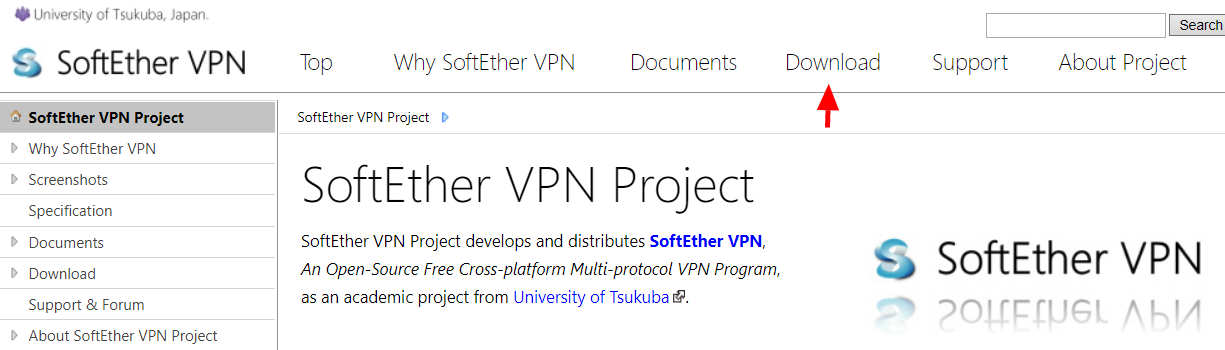
\includegraphics[width=0.6\textwidth]{SoftEther/korak1}
\end{figure}
\FloatBarrier
Odabirom ``Download'' iz izborne trake prikazuje se stranica s ponuđenim poveznicama za preuzimanje.
\begin{figure}[h!]
     \centering
     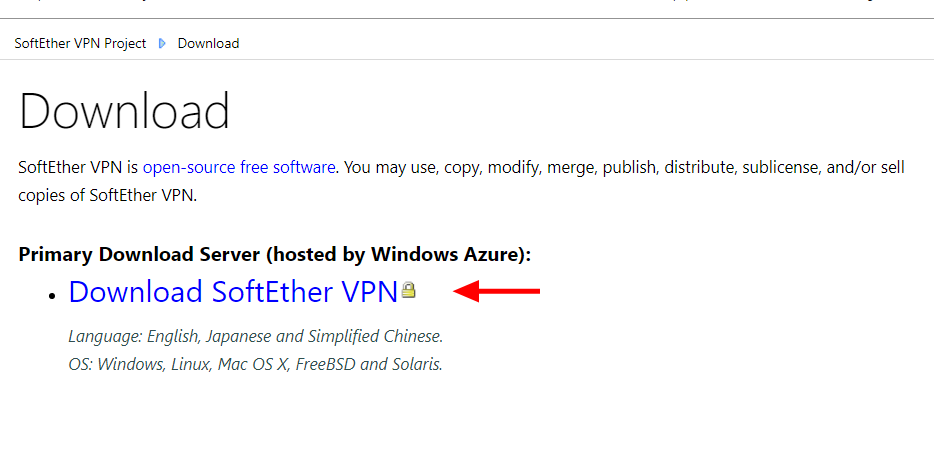
\includegraphics[width=0.6\textwidth]{SoftEther/korak2}
\end{figure}
\FloatBarrier
Sljedeći isječak prikazuje stranicu koja se otvori odabirom prve poveznice. Na stranici se nalaze izborni okviri u kojima je potrebno odabrati željeni program. Za preuzimanje VPN servera potrebno je odabrati postavke prikazane na sljedećem isječku te odabrati prvu poveznicu za početak preuzimanja.
\begin{figure}[h!]
     \centering
     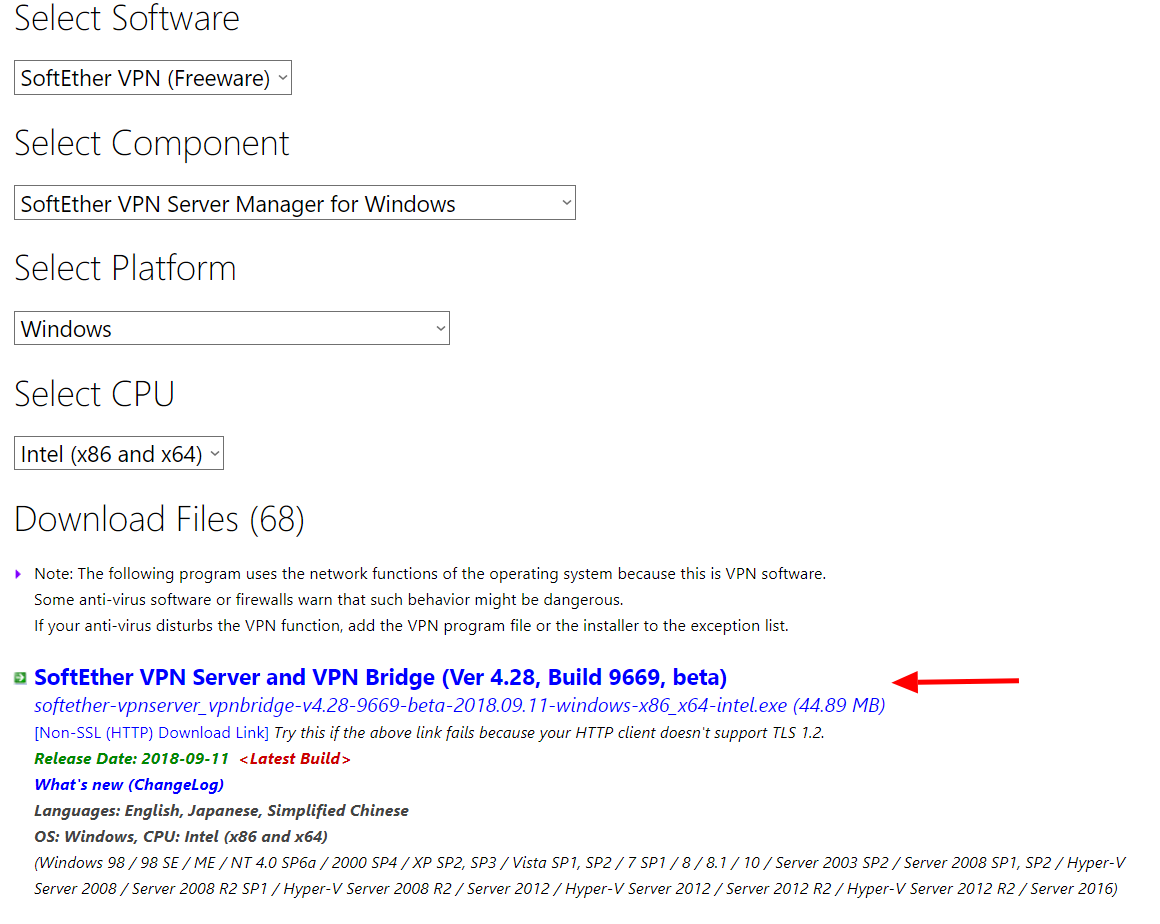
\includegraphics[width=0.6\textwidth]{SoftEther/korak6}
\end{figure}
\FloatBarrier
Nakon preuzimanja i pokretanja instalacije otvara se sljedeći prozor u kojemu se predlaže odabir prvog ponuđenog jer nudi potpunu instalaciju.
\begin{figure}[h!]
     \centering
     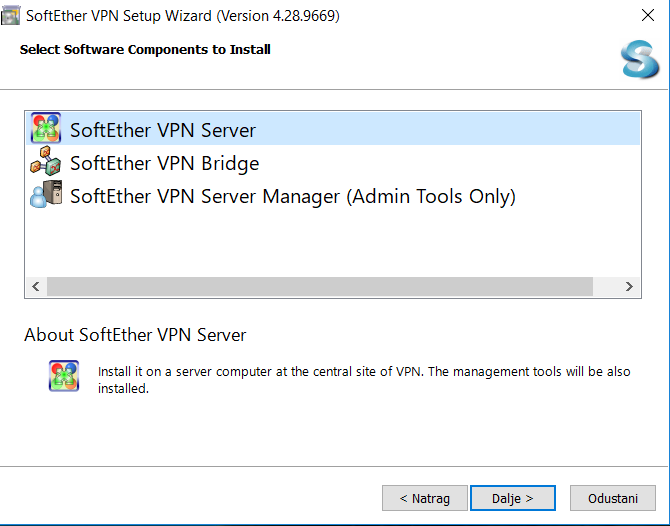
\includegraphics[width=0.6\textwidth]{SoftEther/korak7}
\end{figure}
\FloatBarrier
Nakon uspješne instalacije prikazuje se sljedeći okvir u kojem još nema niti jednog servera. Dodavanje servera započinje se odabirom ``New Setting''.
\begin{figure}[h!]
     \centering
     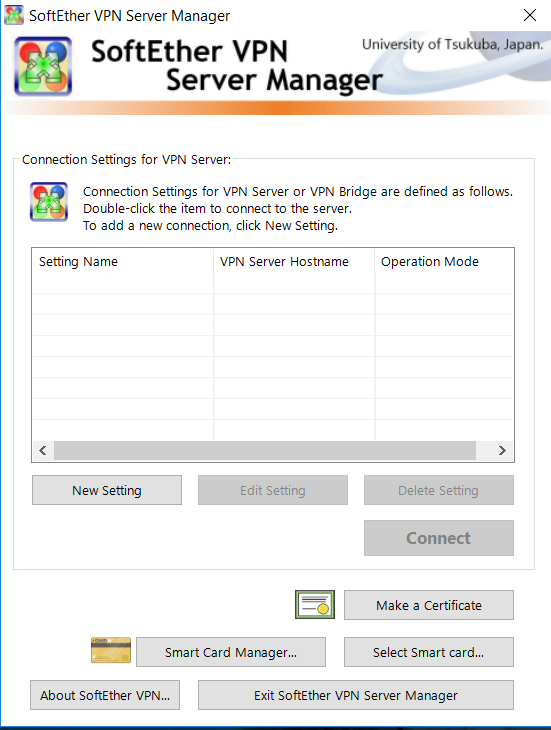
\includegraphics[width=0.6\textwidth]{SoftEther/korak8}
\end{figure}
\FloatBarrier
Stvaranje servera započinje se upisom željenog naziva u polje ``setting name'' i upisom vlastite IP adrese preko koje je trenutno računalo spojeno na Internet. Upute za pronalazak IP adrese mogu se pronaći na kraju ovog poglavlja. Preporuka je dodati lozinku za pristup serveru radi dodatne sigurnosti u polje ``password''.
\begin{figure}[h!]
     \centering
     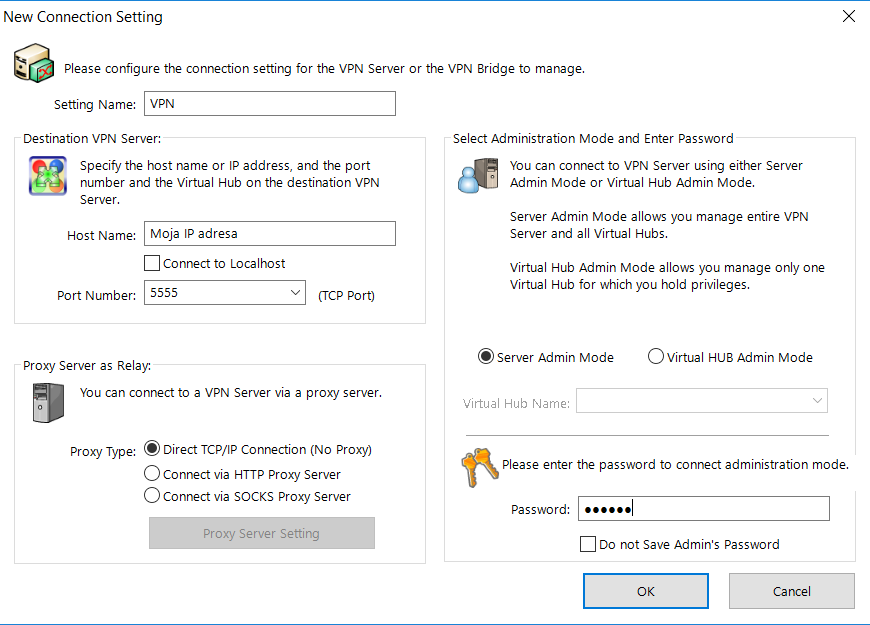
\includegraphics[width=0.6\textwidth]{SoftEther/korak9}
\end{figure}
\FloatBarrier
U tablici sada vidimo da je dodan novi server kojeg je potrebno konfigurirati odabirom ``Connect'' opcije.
\begin{figure}[h!]
     \centering
     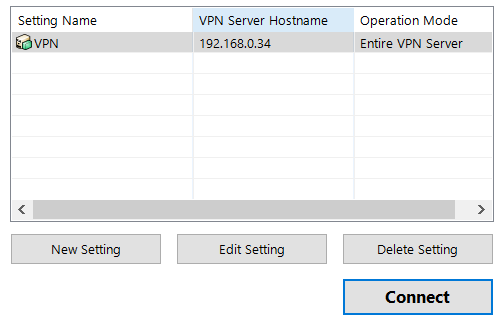
\includegraphics[width=0.6\textwidth]{SoftEther/korak10}
\end{figure}
\FloatBarrier
Kako bi se druga računala uspjela povezati s napravljenim serverom, potrebno je dodati virtualno čvorište odabirom opcije ``Create a Virtual Hub''.
\begin{figure}[h!]
     \centering
     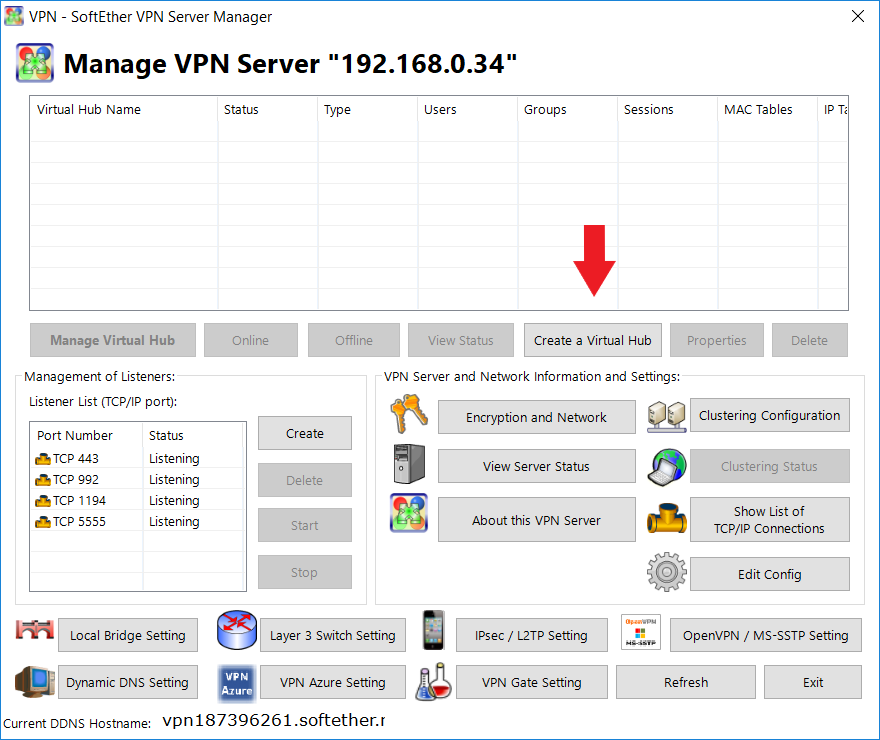
\includegraphics[width=0.6\textwidth]{SoftEther/korak11}
\end{figure}
\FloatBarrier
Virtualnom čvorištu postavljamo proizvoljno ime te dodajemo lozinku radi dodatne sigurnosti.
\begin{figure}[h!]
     \centering
     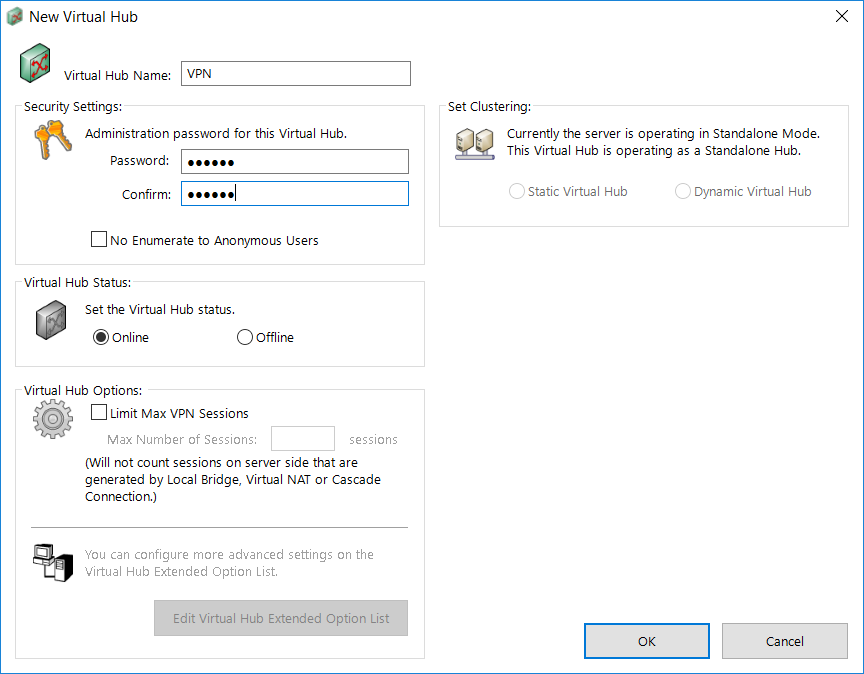
\includegraphics[width=0.6\textwidth]{SoftEther/korak12}
\end{figure}
\FloatBarrier
Sada se može vidjeti novo dodano čvorište u tablici.
\begin{figure}[h!]
     \centering
     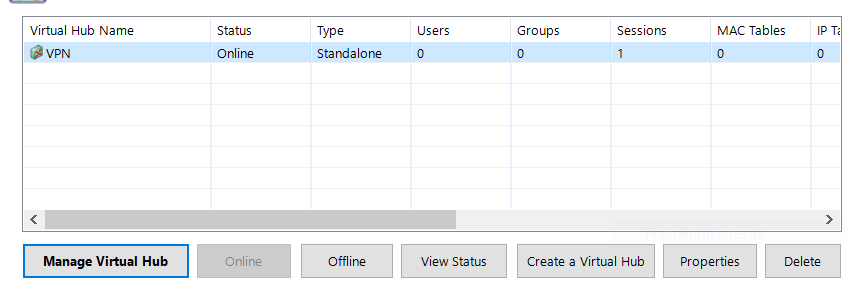
\includegraphics[width=0.6\textwidth]{SoftEther/korak13}
\end{figure}
\FloatBarrier
Sljedeći je korak odrediti tko se sve može povezati na naš server, a to se radi odabirom gumba ``Manage Virtual Hub''.
\begin{figure}[h!]
     \centering
     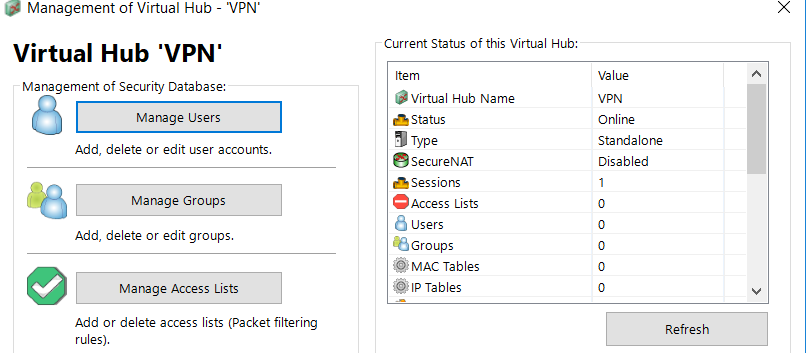
\includegraphics[width=0.6\textwidth]{SoftEther/korak14}
\end{figure}
\FloatBarrier
Na ovom prozoru odabiremo ``Manage Users''.
\begin{figure}[h!]
     \centering
     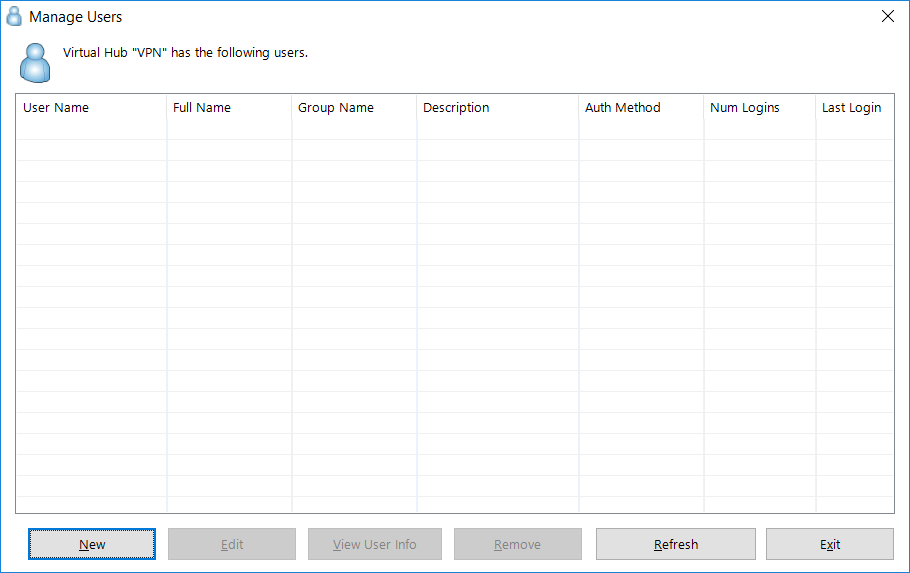
\includegraphics[width=0.4\textwidth]{SoftEther/korak15}
\end{figure}
\FloatBarrier
Sada dodajemo korisnika kojem ćemo dodati proizvoljno ime (u ovim je uputama korisnik nazvan ``klijent1'' i u svim narednim koracima gdje se to ime pojavljuje vama će se pojaviti vaše odabrano ime). Kako bismo smanjili vjerojatnost zlouporabe VPN-a, odabiremo mogućnost prijave klijenta uporabom našeg certifikata i lozinke. Zbog toga odabiremo ``Create Certificate''.
\begin{figure}[h!]
     \centering
     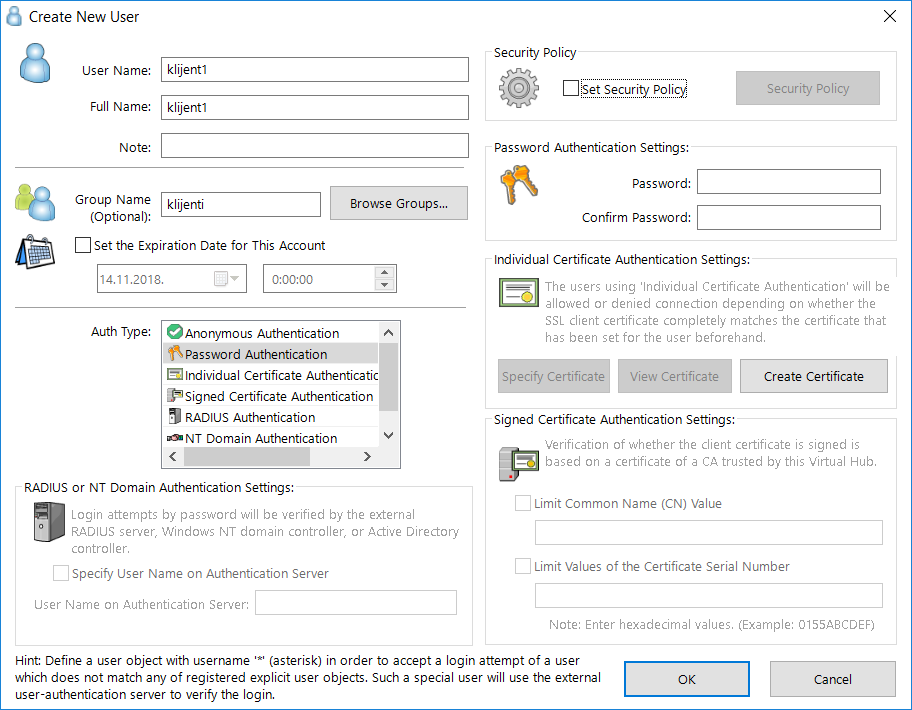
\includegraphics[width=0.6\textwidth]{SoftEther/korak16}
\end{figure}
\FloatBarrier
U sljedećim je poljima moguće detaljno odrediti opis stvorenog klijenta kao i vrijeme njegovog postojanja.
\begin{figure}[h!]
     \centering
     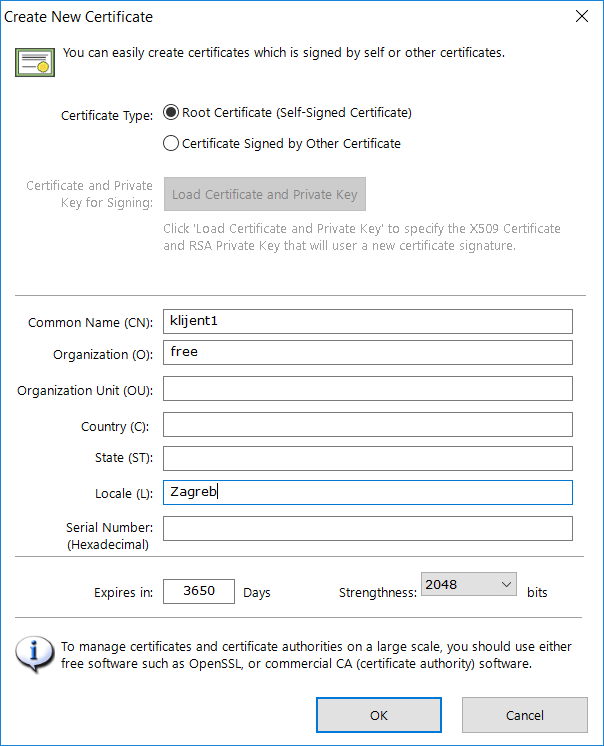
\includegraphics[width=0.6\textwidth]{SoftEther/korak17}
\end{figure}
\FloatBarrier
Nakon otvaranja ovog prozora postavljamo lozinku kojom će se naš klijent prijavljivati na server i koja će samo njemu biti poznata.
\begin{figure}[h!]
     \centering
     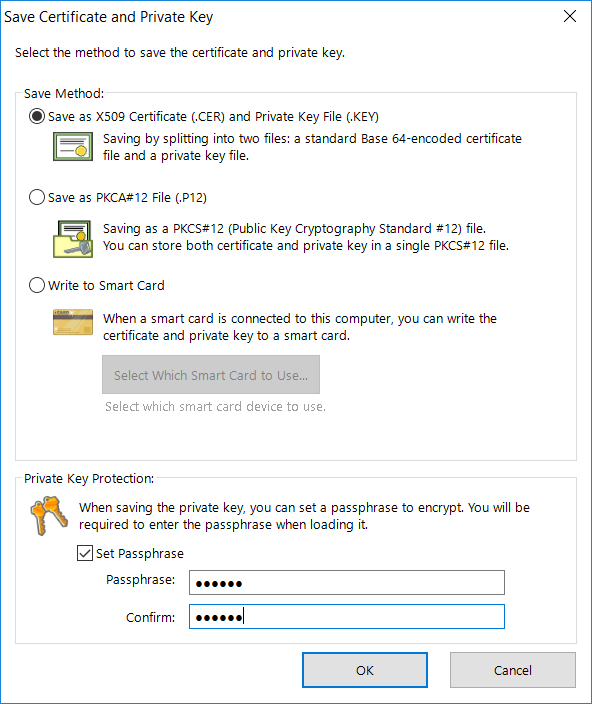
\includegraphics[width=0.6\textwidth]{SoftEther/korak18}
\end{figure}
\FloatBarrier
Nakon potvrde nastaju dvije datoteke: jedna je .cer, a druga je .key i obje su neophodne za prijavu na naš server zato ih mi moramo spremiti i prebaciti na računala koja će se htjeti povezati na server. Povezivanje na server objašnjeno je u jednom od sljedećih dijelova poglavlja.
\begin{figure}[h!]
     \centering
     
\includegraphics[width=0.3\textwidth]{SoftEther/korak20}
\end{figure}
\FloatBarrier
Nakon potvrde vidljiv je korisnik koji se može spojiti na naš server. Moguće je naravno dodavanje više različitih korisnika i brisanje istih.
\begin{figure}[h!]
     \centering
     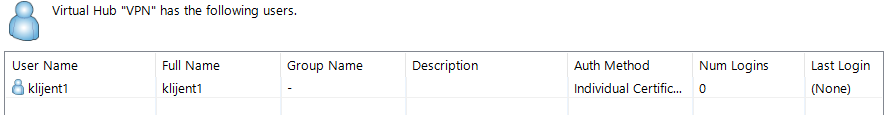
\includegraphics[width=0.6\textwidth]{SoftEther/korak19}
\end{figure}
\FloatBarrier

\newpage
\paragraph*{Instalacija SoftEther klijenta}

\hfill \smallbreak
Za razliku od instalacije i konfiguracije servera, instalacija je SoftEther klijenta jednostavnija. Prvi je korak preuzimanje instalacije sa službene stranice SoftEthera:\\ \url{https://www.softether.org}
\begin{figure}[h!]
	\centering
     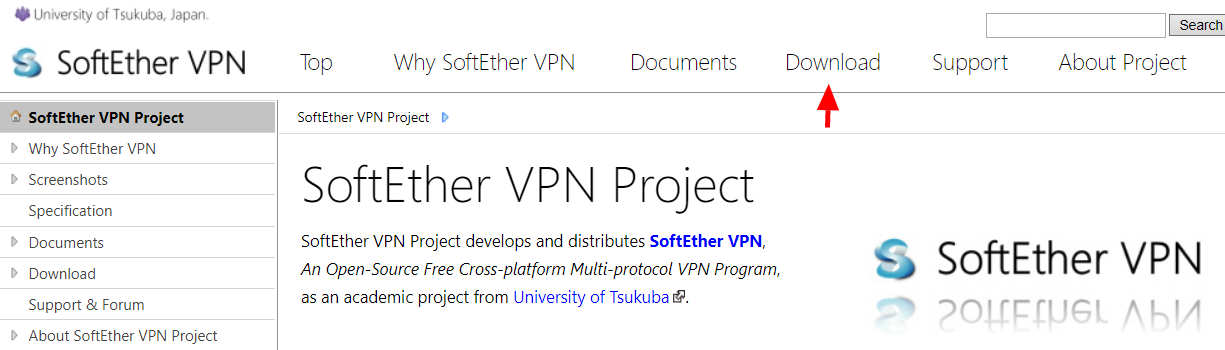
\includegraphics[width=0.6\textwidth]{SoftEther/korak1}
\end{figure}
\FloatBarrier
Odabirom ``Download'' iz izborne trake prikazuje se stranica s ponuđenim poveznicama za preuzimanje.
\begin{figure}[h!]
     \centering
     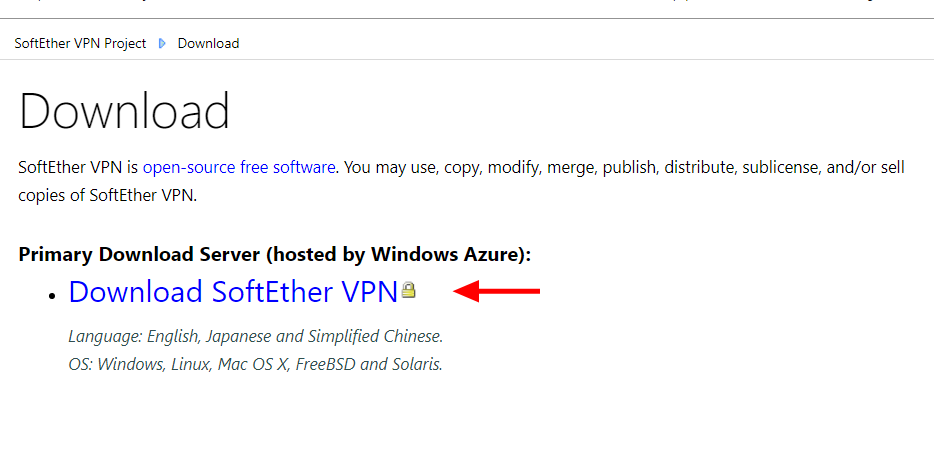
\includegraphics[width=0.6\textwidth]{SoftEther/korak2}
\end{figure}
\FloatBarrier
Sljedeći isječak prikazuje stranicu koja se otvori odabirom prve poveznice. Na stranici se nalaze izborni okviri u kojima je potrebno odabrati željeni program. Za preuzimanje VPN klijenta potrebno je odabrati postavke prikazane na sljedećem isječku te odabrati prvu poveznicu za početak preuzimanja.
\begin{figure}[h!]
     \centering
     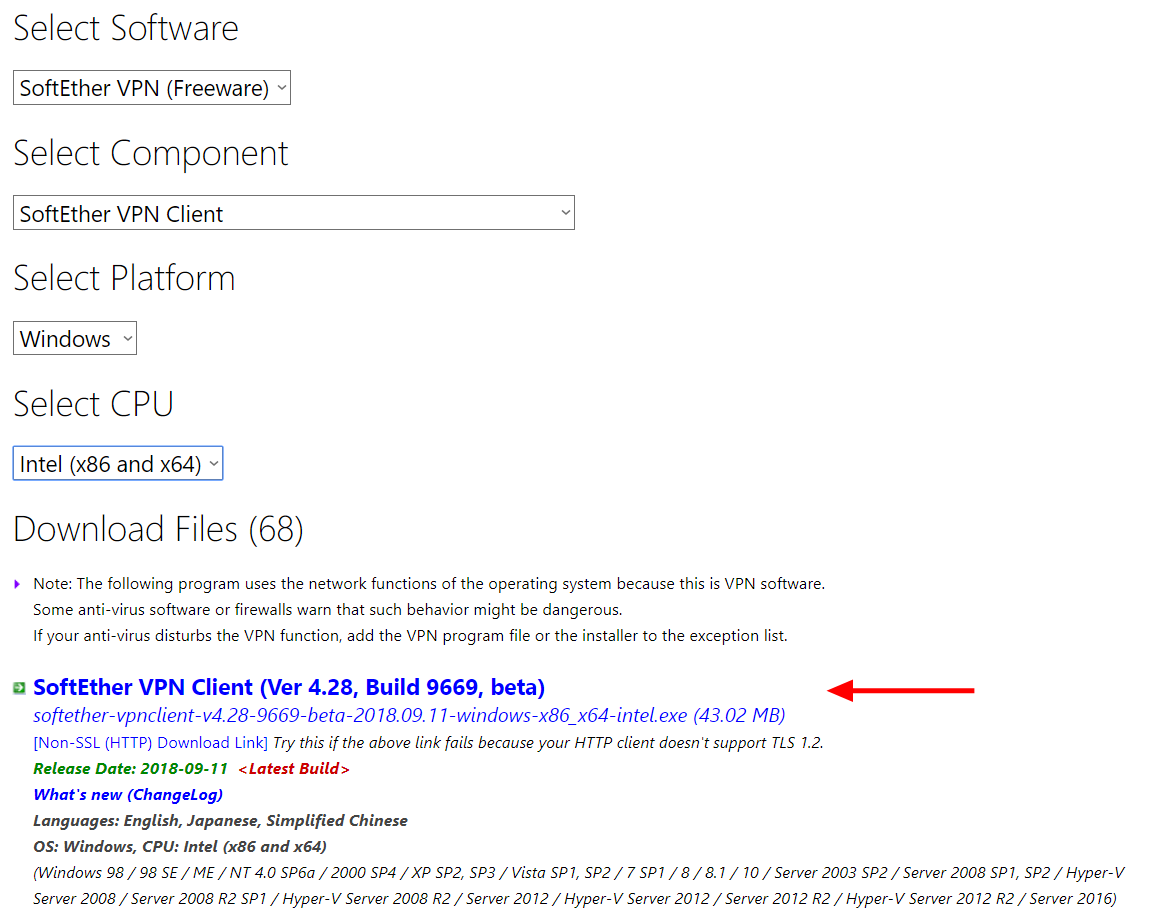
\includegraphics[width=0.6\textwidth]{SoftEther/korak3}
\end{figure}
\FloatBarrier
Nakon završetka preuzimanja i pokretanja instalacije prikazuje se sljedeći prozor. Preporuka je odabrati prvo ponuđeno jer nudi potpunu instalaciju programa.
\begin{figure}[h!]
     \centering
     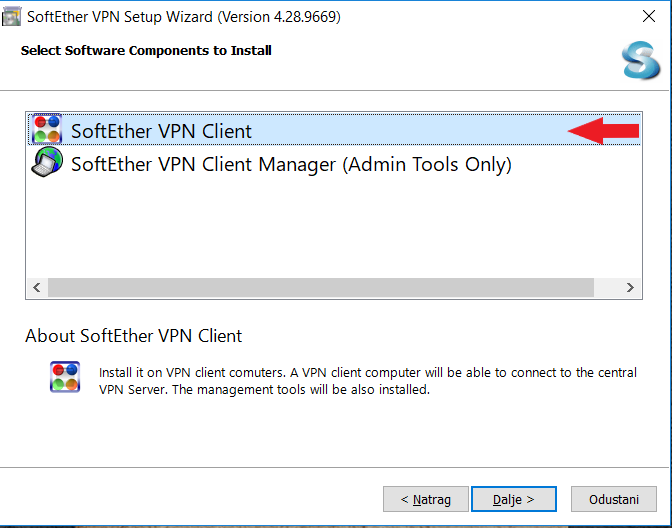
\includegraphics[width=0.6\textwidth]{SoftEther/korak4}
\end{figure}
\FloatBarrier
Ukoliko je instalacija uspješno završena, prikazuje se sljedeći prozor.
\begin{figure}[h!]
     \centering
     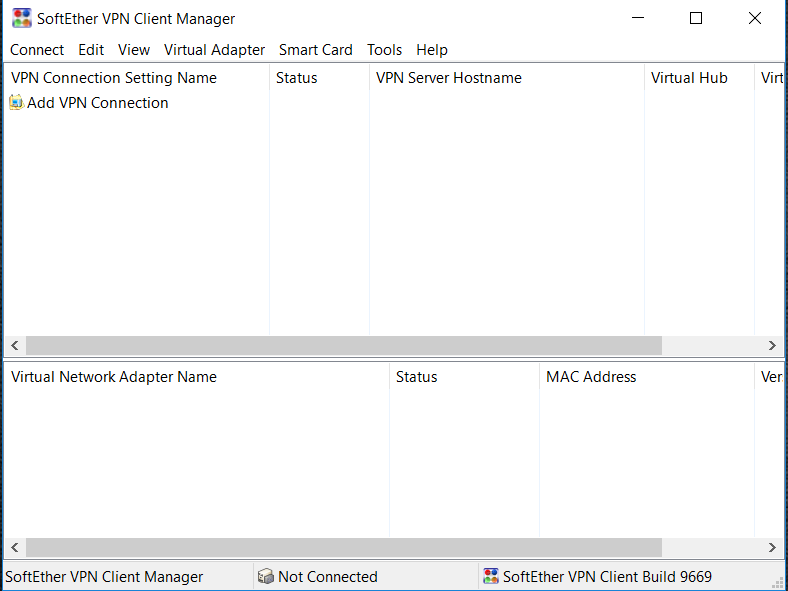
\includegraphics[width=0.6\textwidth]{SoftEther/korak5}
\end{figure}
\FloatBarrier

\newpage
\paragraph*{Povezivanje klijenta sa SoftEther serverom}

\hfill \smallbreak
Za uspješno povezivanje s napravljenim serverom potrebno je pokrenuti aplikaciju SoftEether VPN Client i odabrati opciju dodavanja novog VPN-a. Ako nije postavljen virtualni mrežni adapter, kao što je prikazano u sljedećem primjeru, potrebno je stvoriti novi. Prikazano je stvaranje VPN adaptera.
\begin{figure}[h!]
     \centering
     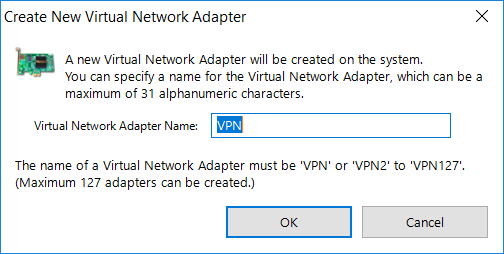
\includegraphics[width=0.6\textwidth]{SoftEther/korak21}
\end{figure}
\FloatBarrier
Nakon stvaranja adaptera moramo dodati server na koji se želimo povezati. Na slici je prikazano stvaranje veze koja se zove VPN. Slično kao i kod stvaranja servera, potrebno je upisati IP adresu preko koje se može serveru pristupiti u polje ``Host name''. Aplikacija nakon upisa IP adrese dohvaća portove na koje se moguće spojiti. Izbor je nekog od ponuđenih portova proizvoljan, kao i postojećih virtualnih mrežnih adaptera. Budući da smo prilikom stvaranja korisnika servera odabrali da se on može prijaviti samo uporabom certifikata i pripadnog ključa, potrebno je stvorene datoteke ``klijent1.cer'' i ``klijent1.key'' prebaciti na računalo s kojeg se pokušava povezati na server. Učitavanje certifikata i ključa u aplikaciju obavlja se odabirom opcije ``specify client certificate''.
\begin{figure}[h!]
     \centering
     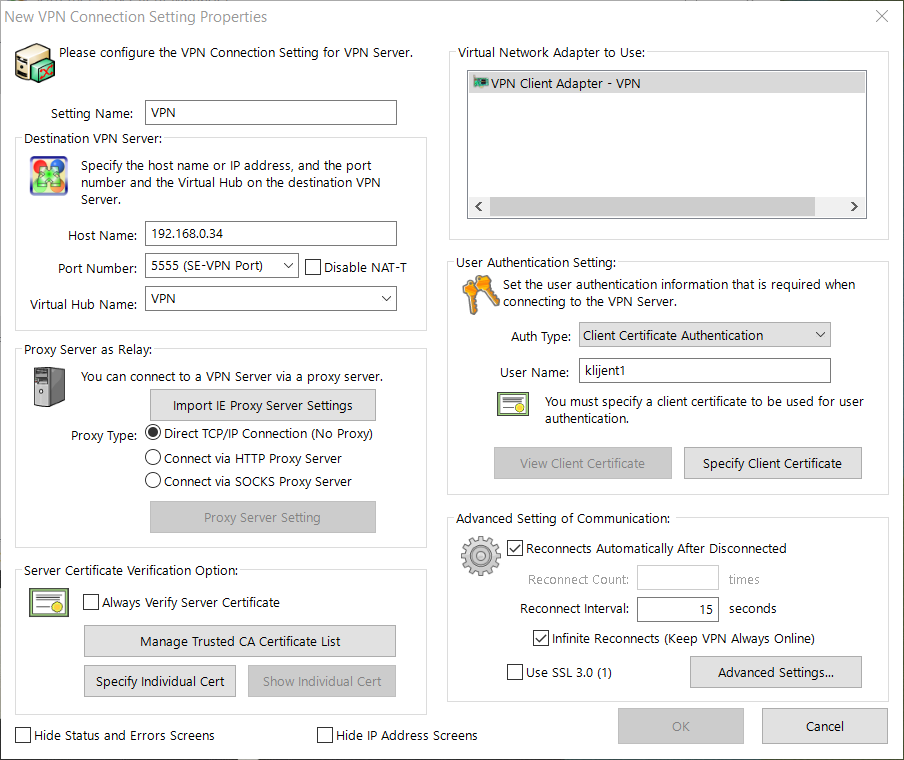
\includegraphics[width=0.6\textwidth]{SoftEther/korak22}
\end{figure}
\FloatBarrier
Nakon učitavanja datoteka prikazuje se prozor sa sljedećeg isječka u koji se upisuje lozinka koju smo postavili prilikom stvaranja klijenta.
\begin{figure}[h!]
     \centering
     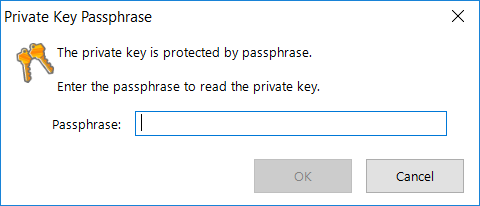
\includegraphics[width=0.6\textwidth]{SoftEther/korak23}
\end{figure}
\FloatBarrier
Ako smo učitali ispravni certifikat i unijeli ispravnu lozinku, tada će se prikazati prozor na kojem vidimo povezivanje s VPN serverom.
\begin{figure}[h!]
     \centering
     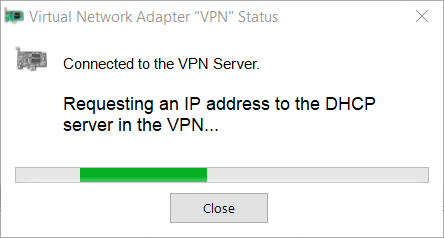
\includegraphics[width=0.5\textwidth]{SoftEther/korak24}
\end{figure}
\FloatBarrier

\FloatBarrier

\subsubsection{Provjera vlastite IP adrese}
\hfill \smallbreak
Kako bi server bio uspješno uspostavljen, potrebna mu je IP adresa dodijeljena računalu na kojem se nalazi. Najbrži način na koji se ona može odrediti jest otvaranje naredbenog retka i upis naredbe IPCONFIG. Rezultat te naredbe bit će prikaz mrežnih postavki za trenutno aktivne mrežne adaptere.
Crvenom je strelicom označena IP adresa na trenutno aktivnom adapteru.
\begin{figure}[h!]
     \centering
     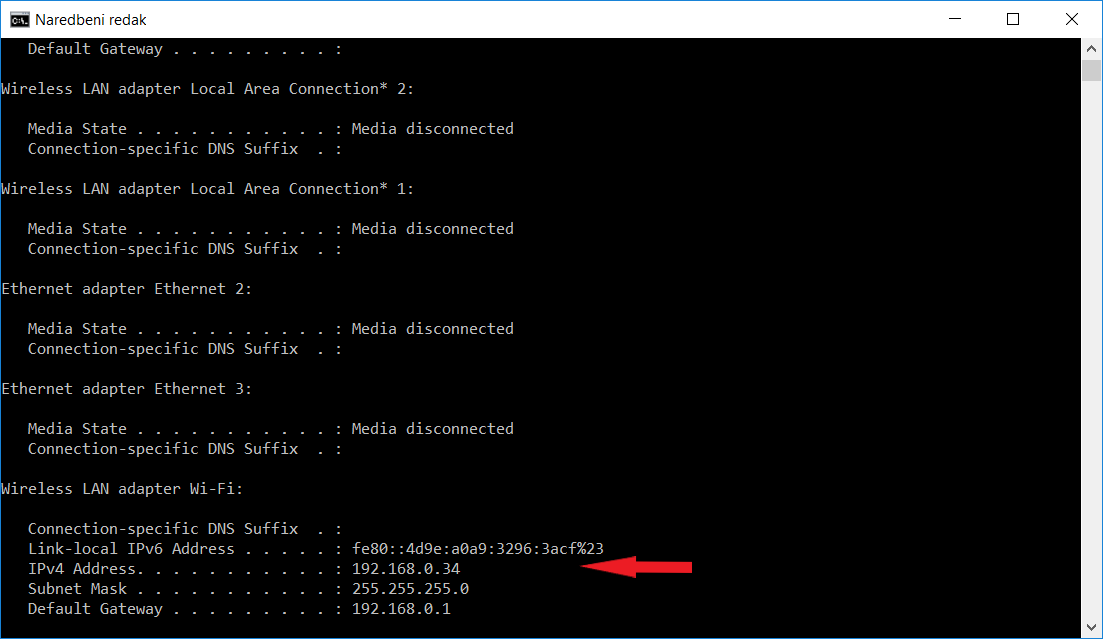
\includegraphics[width=0.6\textwidth]{SoftEther/IP1}
\end{figure}
\FloatBarrier

% za usporedbu === https://www.softether.org/@api/deki/files/12/=1.3.jpg
% pomoć pri instalaciji === https://www.youtube.com/watch?v=VbvRhPqNCsk
	
	\newpage
	\subsubsection{Tinc}
	\hfill \smallbreak
Tinc je još jedan besplatan program za uspostavu VPN veze. Ono po čemu se tinc razlikuje od drugih programa je niz jedinstvenih mogućnosti koje uključuje, kao što su enkripcija, neobavezna kompresija, automatsko usmjeravanje u mreži „svatko sa svakim“, lagano proširivanje… Ove mogućnosti čine tinc jako dobrim rješenjem za poslovne mreže koje su sastavljene od velikog broja manjih udaljenih mreža. Slijede upute za instalaciju, konfiguraciju i pokretanje tinc-a.

\subparagraph{Instalacija}
\hfill \smallbreak
Prvo preuzmemo instalacijski paket s adrese 
\url{http://www.tinc-vpn.org/packages/windows/tinc-1.1pre15-install.exe} te obavimo standardi instalacijski postupak, pokrenemo installer, next, prihvatimo uvjete korištenja, Ok, označimo sva polja kada nas pita koje komponente želimo instalirati, next, install, finish. \\Slijedi postupak za postavljanje računala poslužitelja, ovaj postupak radimo na računalu koje se nalazi u mreži kojoj želimo pristupati koristeći udaljeno računalo klijent. Otvorimo mapu u koju smo instalirali tinc (vjerojatno C:\textbackslash Program Files\textbackslash tinc) unutar komandne linije koju smo pokrenuli kao administrator, pozicioniramo se u mapu C:\textbackslash Program Files\textbackslash tinc te upisujemo redom naredbe (u zagradama se nalaze komentari, njih ne upisujemo u komandnu liniju):
\FloatBarrier
\smallbreak \code{tinc -n vpn init master}
\smallbreak \code{tinc -n vpn add subnet 20.0.1.1} (dodjela ip-adrese koju želimo da ima, na primjer 20.0.1.1)
\smallbreak \code{tinc -n vpn add address=FQDNORIP}  (gdje je FQDNORIP javna IP adresa poslužiteljskog računala)
\smallbreak \code{cd tap-win64}
\smallbreak \code{addtap.bat}
\smallbreak \code{cd ..}
\smallbreak \code{netsh interface ipv4 show interfaces}  (pogledamo što je odspojeno, vjerojatno Ethernet 2)
\smallbreak \code{netsh interface set interface name = "Ethernet 2" newname = "tinc"}
\smallbreak \code{netsh interface ip set address "tinc" static 20.0.1.1    255.255.255.0}
\smallbreak \code{netsh interface ipv4 show config}  (sada bi trebali imati sučelje „tinc“ s maskom podmreže i IP-adresom)\\
\FloatBarrier
Time je konfiguriran poslužitelj. Sada sličan postupak moramo ponoviti za računalo klijent. Na njemu također nakon instalacije pokrenemo komandnu liniju kao administrator i pozicioniramo se u mapu gdje je tinc instaliran te upišemo sljedeće naredbe:
\FloatBarrier
\smallbreak \code{tinc -n vpn init client1}
\smallbreak \code{tinc -n vpn add connectto master}
\smallbreak \code{tinc -n vpn add subnet 20.0.2.2}
\smallbreak \code{cd tap-win64}
\smallbreak \code{addtap.bat}
\smallbreak \code{cd ..}
\smallbreak \code{netsh interface ipv4 show interfaces}  (pogledamo što je odspojeno, vjerojatno Ethernet 2)
\smallbreak \code{netsh interface set interface name = "Ethernet 2" newname = "tinc"}
\smallbreak \code{netsh interface ip set address "tinc" static 20.0.2.2 255.255.255.0}\\
\FloatBarrier
Potrebno je još samo s klijentskog računala kopirati datoteku vpn/hosts/client1 na poslužiteljsko računalo u mapu vpn/hosts
i s poslužiteljskog računala kopirati datoteku vpn/hosts/master na klijentsko računalo u mapu vpn/hosts. Sada je sve spremno za korištenje.

\subparagraph{Pokretanje}
\hfill \smallbreak
Kada je završena instalacija i konfiguracija, mreža će izgledati kao mreža sa slike 41., a tinc se pokrene jednostavnom naredbom koja je jednaka za klijenta i poslužitelja:
\FloatBarrier
\smallbreak \code{tincd -n vpn -D -d3}
\FloatBarrier
\begin{figure}[h!]
	\centering
     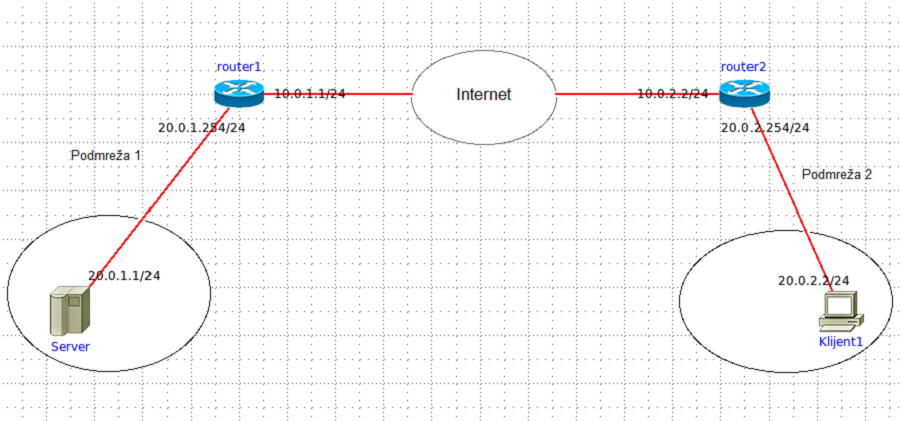
\includegraphics[width=0.8\textwidth]{Tinc/Slika41}
     \caption{Izgled mreže nakon uspostave VPN-a}
\end{figure}
\FloatBarrier
	
	\newpage
	\subsubsection{OpenVPN za Windows}
	\bigbreak
\paragraph*{Ukratko o OpenVPN tehnologiji}
\hfill \smallbreak

OpenVPN\cite{openvpn} besplatan je program za ostvarenje vlastitog virtualnog privatnog tunela preko interneta. OpenVPN-om možemo ostvariti brojna rješenja povezivanja kao što su prijenos podataka, uporaba servera kao pristupne točke na internet, povezivanje udaljenih uređaja u logičku LAN mrežu,...\smallbreak
Neke svojstva OpenVPN povezivanja:
\begin{itemize}
	\item sigurni virtualni tunel na internetu
	\item prijenos podataka TCP ili UDP protokolom
	\item odabir željene vrste šifriranja
	\item višestruko povezivanje
	\item povezivanje računala s različitim operacijskim sustavima
\end{itemize}
\smallbreak
Topologija koja se želi u ovom poglavlju ostvariti jest priključivanje korisnika udaljenoj mreži kao što je ilustrirano na slici \ref{fig:topologija-open}. Korisnik će preko svojeg računala uspostaviti virtualni privatni tunel preko Interneta s računalom koje ima instaliran i konfiguriran OpenVPN server. Nakon povezivanja će korisnik pripadati logičkoj lokalnoj mreži servera.
\begin{figure}[h!]
	\centering
     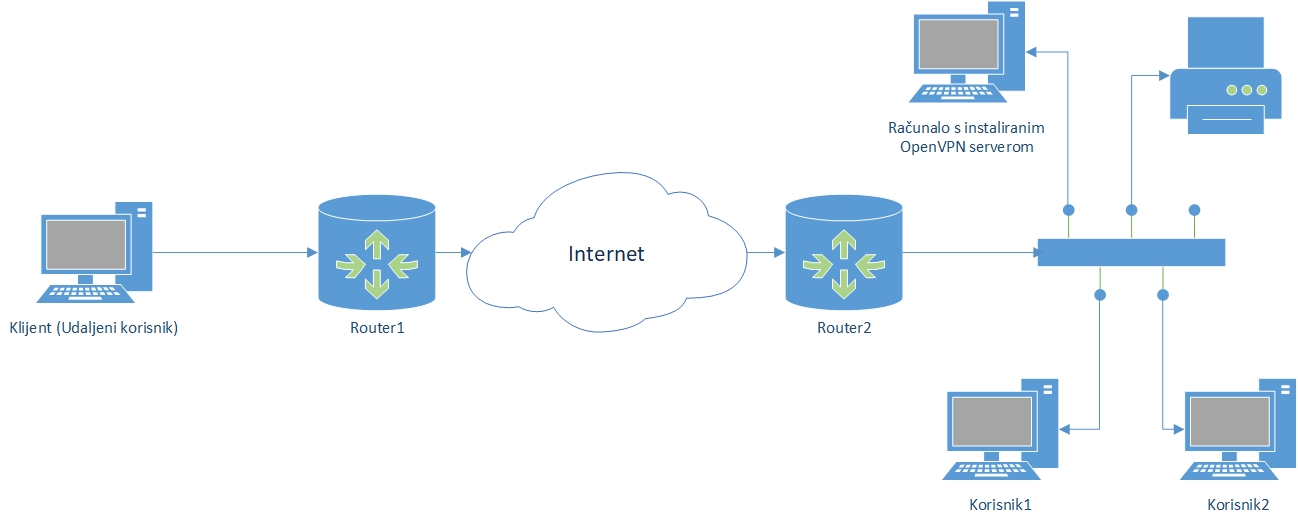
\includegraphics[width=0.9\textwidth]{OVPN-win/topologija}
     \caption{VPN topologija}
     \label{fig:topologija-open}
\end{figure}
\FloatBarrier
\bigbreak
\paragraph*{Instalacija OpenVPN servera}
\hfill \bigbreak
Za početak potrebno je preuzeti instalaciju VPN-a sa službene stranice OpenVPN-a:\\ \url{https://openvpn.net/community-downloads/}
\hfill \smallbreak
Na službenoj stranici potrebno je pokrenuti preuzimanje verzije za operacijski sustav Windows:
\begin{figure}[h!]
	\centering
     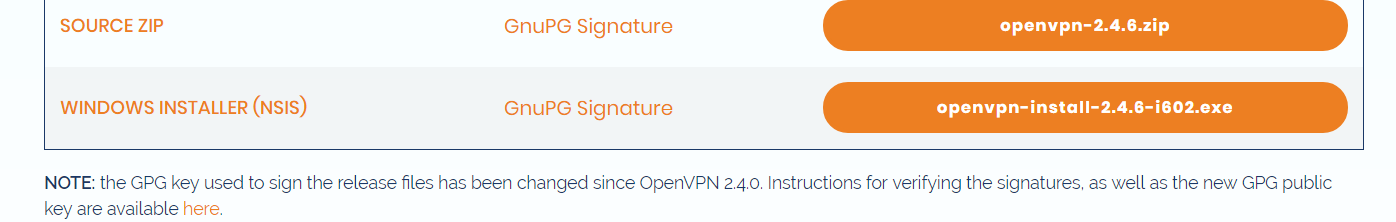
\includegraphics[width=0.8\textwidth]{OVPN-win/slika1}
     \caption{Prikaz poveznice za preuzimanje}
\end{figure}
\FloatBarrier
\begin{wrapfigure}{r}{0.4\textwidth}
  \begin{center}
    
\includegraphics[width=0.2\textwidth]{OVPN-win/slika2}
    \caption{Ikona instalacije}
  \end{center}
\end{wrapfigure}
\FloatBarrier
Ako je uspješno obavljeno preuzimanje, može se započeti instalacija pokretanjem programa s ovakvom ikonom.
\bigbreak
Dalje je potrebno pratiti klasične korake instalacije programa. Kada vam program ponudi odabir direktorija instalacije, preporuka je da odaberete pretpostavljeni direktorij jer su daljnje upute i konfiguracija pravljeni prema tom uzoru. Ako odaberete vlastiti, morate puteve prikazane u daljnjim koracima preoblikovati tako da vode do vašeg direktorija instalacije.
\smallbreak

Obratite pažnju na sljedeću sliku (slika \ref{fig:instalacija-open}) jer prikazuje uz pretpostavljene i važan odabir za uspješnu instalaciju. Potrebno je odabrati i instalirati ``EasyRSA 2 Certificate Management Scripts''.
\begin{figure}[h!]
	\centering
     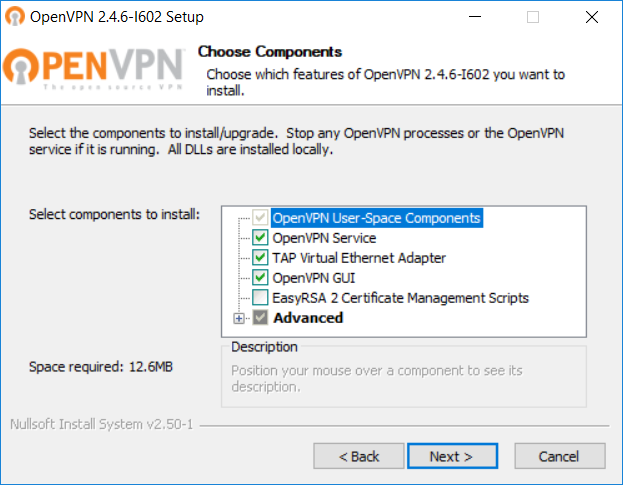
\includegraphics[width=0.7\textwidth]{OVPN-win/slika3}
     \caption{Prikaz dodataka instalacije}
     \label{fig:instalacija-open}
\end{figure}
\FloatBarrier
U sklopu instalacije programa obavljena je i instalacija virtualnog mrežnog priključka na računalu. Taj će se priključak koristiti za povezivanje poslužitelja i klijenata te je vidljiv u postavkama mreže računala:\smallbreak
\small\textcolor{blue}{Upravljačka ploča/Sve stavke upravljačke ploče/Mrežne veze}
\smallbreak
Kako bismo ga lakše adresirali kasnije, promijenit ćemo mu ime u ``ServerVPN''. Adapter se razlikuje od ostalih jer mu je opis ``TAP-Windows Adapter V9''.

\begin{figure}[h!]
    \centering
    \begin{subfigure}[b]{0.35\textwidth}
        
\includegraphics[width=\textwidth]{OVPN-win/slika4}
        \caption{Prije}
        \label{fig:prije}
    \end{subfigure}
    $\Longrightarrow$
    \begin{subfigure}[b]{0.35\textwidth}
        
\includegraphics[width=\textwidth]{OVPN-win/slika5}
        \caption{Nakon}
        \label{fig:nakon}
    \end{subfigure}
    \caption{Preimenovanje TAP adaptera}
\end{figure}
\FloatBarrier

Naredni se koraci izvode upisom naredbi u naredbeni redak. Potrebno je naredbeni redak pokrenuti kao administrator za što je prikazan jedan od mogućih načina na slici \ref{fig:administrator-win}.

\begin{figure}[h!]
	\centering
     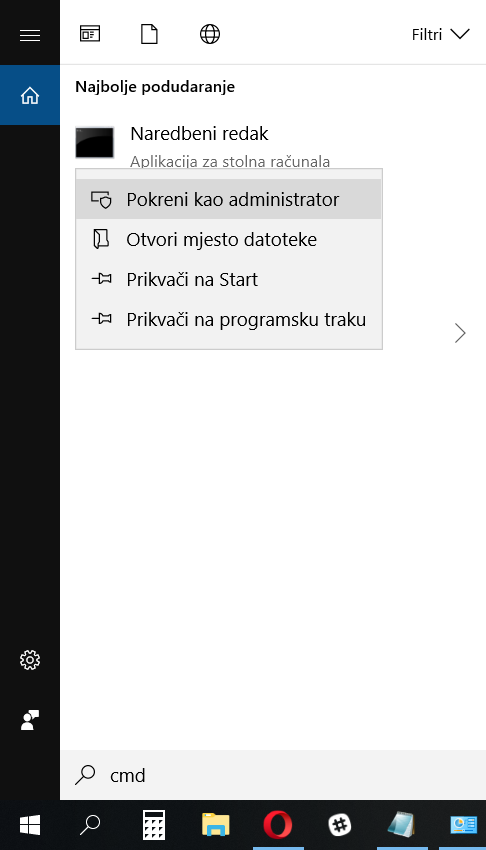
\includegraphics[width=0.4\textwidth]{OVPN-win/slika6}
     \caption{Pokretanje naredbenog retka u administratorskom načinu}
     \label{fig:administrator-win}
\end{figure}
\FloatBarrier

Potrebno se pozicionirati u ``easy-rsa'' direktorij u instalacijskom direktoriju upisom naredbe:
\begin{lstlisting}
cd "C:\Program Files\OpenVPN\easy-rsa"
\end{lstlisting}
Sada je potrebno upisivati po redu sljedeće naredbe.
\begin{lstlisting}
init-config.bat
\end{lstlisting}
Naredba inicijalizira konfiguracijsku datoteku u kojoj možemo dodati informacije o vezi koju uspostavljamo. Ti podaci neće utjecati na rad servera i klijenata.
\begin{lstlisting}
vars
clean-all
build-dh
\end{lstlisting}

\begin{figure}[h!]
	\centering
     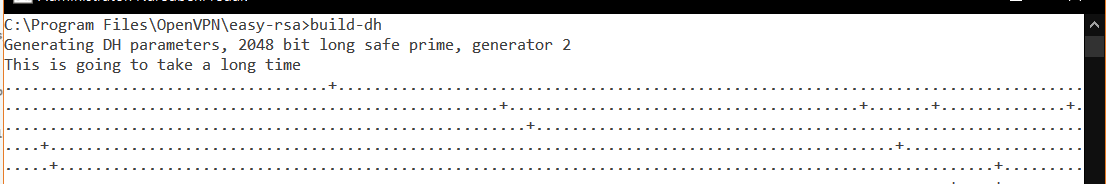
\includegraphics[width=0.9\textwidth]{OVPN-win/slika10}
     \caption{Prikaz pokretanja build-dh naredbe}
\end{figure}
\FloatBarrier
Naredbom se stvara potrebna ``.dh'' datoteka. Na nekim inačicama operacijskog sustava Windows moguća je greška: ``openssl" is not recognized ...\smallbreak
U tom slučaju otići u napredne postavke sustava i dodati ``PATH'' varijablu, tj. put do bin datoteke OpenVPN-a :
\small\textcolor{blue}{C:\textbackslash Program Files\textbackslash OpenVPN\textbackslash bin}
\begin{lstlisting}
build-ca
\end{lstlisting}
Ovom je naredbom započeto stvaranje certifikata potrebnih za sigurno povezivanje servera i klijenata. Prilikom izvršavanja naredbe program nudi polja koja je potrebno popuniti, tj. informacije o našem serveru kako bi se ugradile u ključ što je vidljivo na slici \ref{fig:ca-open}.
\begin{figure}[h!]
	\centering
     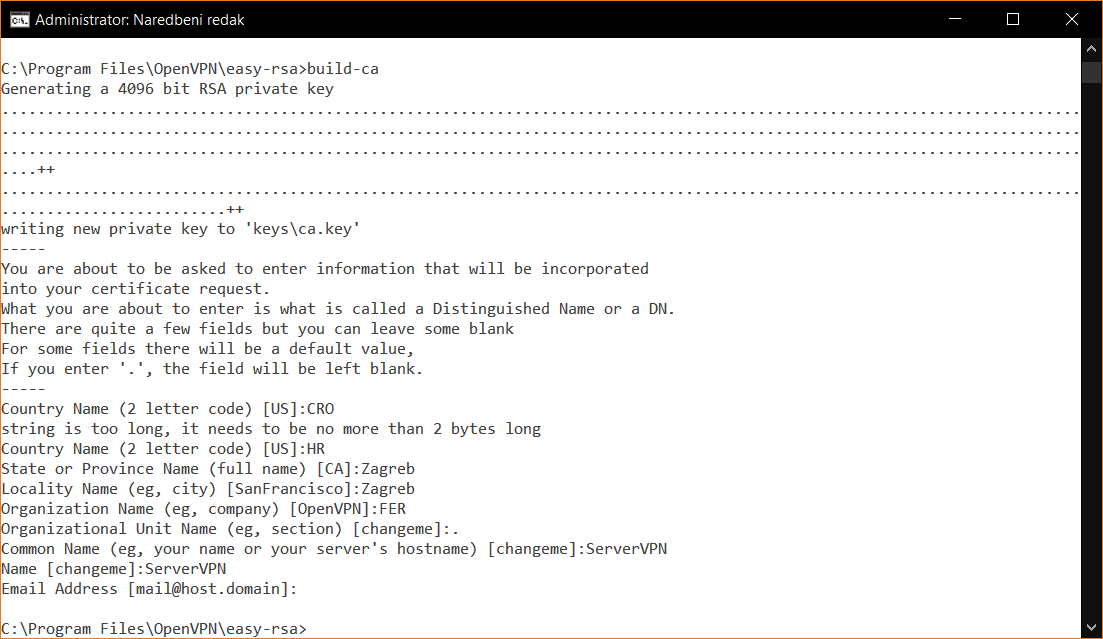
\includegraphics[width=0.9\textwidth]{OVPN-win/slika11}
     \caption{Stvaranje certifikata povezivanja}
     \label{fig:ca-open}
\end{figure}
\FloatBarrier
\begin{lstlisting}
build-key-server ServerVPN
\end{lstlisting}
Ova naredba također nudi upis podataka kao što je vidljivo na slici \ref{fig:serverca-open}, ali ovdje su polja ostavljena prazna jer nisu ključna za rad. Naredbom su nastale 3 datoteke u instalacijskom direktoriju ``.crt'',  ``.csr'' i ``.key''.
\begin{figure}[h!]
	\centering
     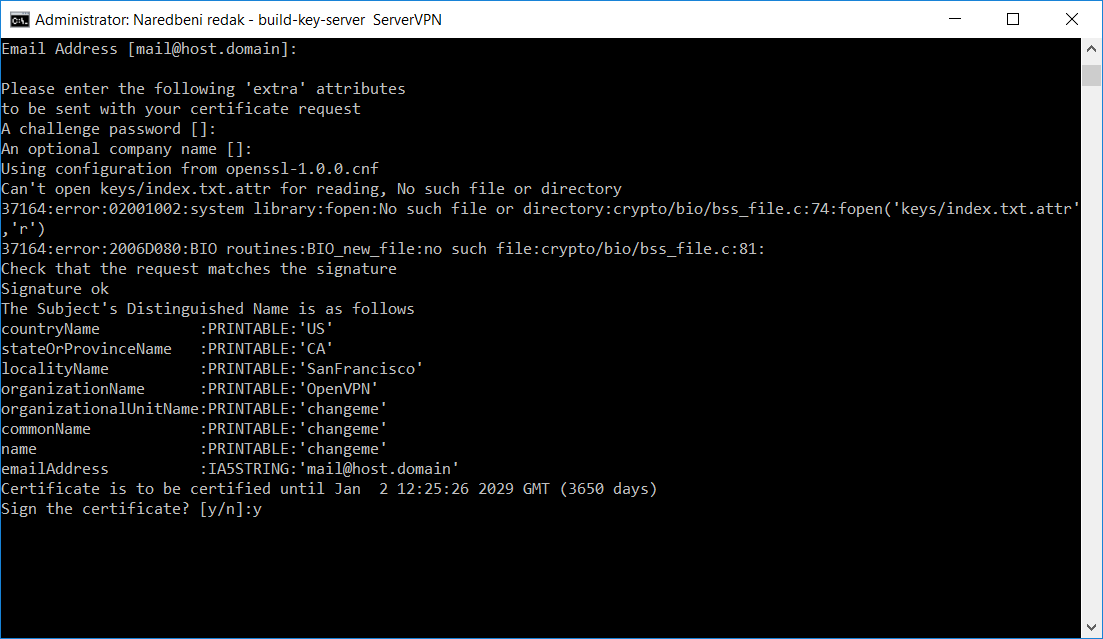
\includegraphics[width=0.9\textwidth]{OVPN-win/slika12}
     \caption{Stvaranje certifikata servera}
     \label{fig:serverca-open}
\end{figure}
\FloatBarrier
Idući korak stvaranje je certifikata klijenta.
\begin{lstlisting}
build-key KlijentVPN
\end{lstlisting}
Po potrebi popuniti podacima o klijentu. Kako bi se razlikovao od ostalih, važno je popuniti polje ``Common Name'' kao na slici \ref{fig:klijent-open} i potvrditi stvaranje.
\begin{figure}[h!]
	\centering
     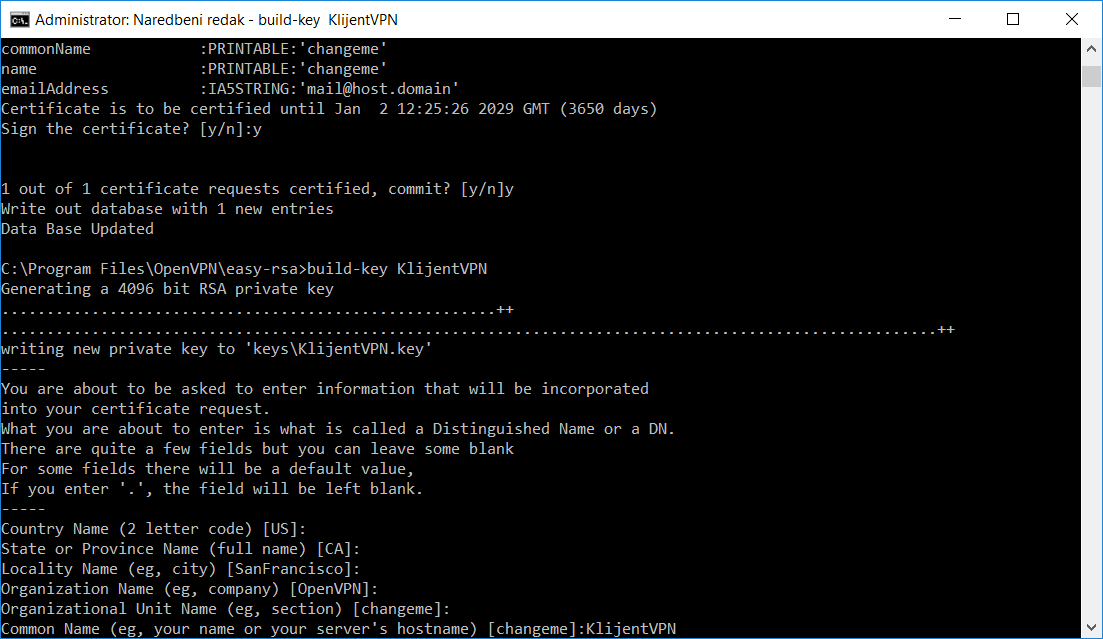
\includegraphics[width=0.9\textwidth]{OVPN-win/slika13}
     \caption{Stvaranje certifikata klijenta}
     \label{fig:klijent-open}
\end{figure}
\FloatBarrier
Kao i u prethodnom koraku nastale su 3 datoteke. Sve su neophodne za prijavu na naš server zato ih mi moramo spremiti i prebaciti na računala koja će se htjeti povezati na server. Povezivanje na server objašnjeno je u jednom od sljedećih dijelova poglavlja.\smallbreak
Moguće je naravno dodavanje više različitih korisnika i brisanje istih.
\begin{lstlisting}
openvpn --genkey --secret keys/ta.key
\end{lstlisting}

Ovom naredbom stvara se ključ kojim se autentificiraju podaci između servera i klijenata.
 
\paragraph*{Konfiguracija OpenVPN servera}
\hfill \bigbreak
Konfiguracijske datoteke ne postoje same po sebi pa ih je potrebno stvoriti na radnoj površini kao prazan tekstualni dokument, spremiti u obliku ``ServerVPN.ovpn'' datoteke pa kopirati u direktorij OpenVPN-a na lokaciju:\smallbreak
\small\textcolor{blue}{C:\textbackslash Program Files\textbackslash OpenVPN\textbackslash config}
\smallbreak

``Server.ovpn'' jest konfiguracijska datoteka stvorenog servera. OpenVPN nudi brojne postavke koje serveru daju širok izbor svojstava i mogućnosti. Naglasak ovih uputa je na povezivanju klijenata i servera te su dodane mogućnosti samo s tim ciljem.\smallbreak
Konfiguracijska datoteka treba sadržavati:\smallbreak
{\small\fontfamily{pcr}\selectfont
dev-node "ServerVPN"\hfill;ime

mode server\hfill;uloga u mreži

port 12345\hfill;vrata preko kojih ide komunikacija	

proto tcp4-server\hfill;protokol prijenosa

dev tun\hfill;stvara se virtualni tunel

tls-server\hfill;za autentifikaciju

tls-auth "C:\textbackslash \textbackslash Program Files\textbackslash \textbackslash OpenVPN\textbackslash \textbackslash easy-rsa\textbackslash \textbackslash keys\textbackslash \textbackslash ta.key" 0\hfill

; put do datoteke ključa(ta.key) te broj 0 koja označava server

tun-mtu 1500\hfill;veličina MTU paketa

tun-mtu-extra 32\hfill;veličina MTU paketa

mssfix 1450\hfill;veličina MTU paketa

ca "C:\textbackslash \textbackslash Program Files\textbackslash \textbackslash OpenVPN\textbackslash \textbackslash easy-rsa\textbackslash \textbackslash keys\textbackslash \textbackslash ca.crt"\hfill

; put do datoteke ca.crt

cert "C:\textbackslash \textbackslash Program Files\textbackslash \textbackslash OpenVPN\textbackslash \textbackslash easy-rsa\textbackslash \textbackslash keys\textbackslash \textbackslash ServerVPN.crt"\hfill

; put do certifikata servera

key "C:\textbackslash \textbackslash Program Files\textbackslash \textbackslash OpenVPN\textbackslash \textbackslash easy-rsa\textbackslash \textbackslash keys\textbackslash \textbackslash ServerVPN.key"\hfill

; put do ključa servera

dh "C:\textbackslash \textbackslash Program Files\textbackslash \textbackslash OpenVPN\textbackslash \textbackslash easy-rsa\textbackslash \textbackslash keys\textbackslash \textbackslash dh2048.pem"\hfill

; put do .dh datoteke

server 10.10.10.0 255.255.255.0\hfill

; virtualna adresa servera i maska podmreže

client-to-client\hfill; klijenti se vide

keepalive 10 120\hfill; vrijeme čekanja na vezu

cipher AES-128-CBC\hfill; vrsta šifriranja

comp-lzo\hfill; kompresija podataka u tunelu

persist-key\hfill;za slučaj prekida veze

persist-tun\hfill;za slučaj prekida veze

client-config-dir "C:\textbackslash \textbackslash Program Files\textbackslash \textbackslash OpenVPN\textbackslash \textbackslash config"\hfill

;direktorij konfiguracije

verb 3\hfill;stupanj ispisa grešaka i upozorenja

route-delay 5\hfill;čekanje do početka primanja zahtjeva

route-method exe\hfill;način unosa rute

push "route 161.53.63.0 255.255.255.0" 

route 161.53.63.204 255.255.255.0\hfill

;adresa koju je router dodijelio računalu na kojem uspostavljamo server
}\bigbreak
Za upute i pojašnjenja kako odabrati ispravne vlastite parametre za ovu datoteku molimo pogledajte detaljnije upute na adresi:\smallbreak \url{https://openvpn.net/community-resources/how-to/\#config}\smallbreak
Osim toga potrebno je:
\begin{itemize}
	\item imati stabilnu vezu na internet i statičku IP adresu
	\item imati omogućenu razmjenu TCP paketa u firewallu
	\item imati omogućeno prosljeđivanje prometa s routera na vrata na kojima server sluša (Port forwarding)
\end{itemize}	
	
Ako je konfiguracija dobro odrađena moguće je pokrenuti server. Povezivanje se započinje pokretanjem ``OpenVPN GUI'' datoteke na radnoj površini, odabirom ikone računala s alatne trake i odabirom ``Connect'' mogućnosti što je prikazano na slici \ref{fig:povezivanje-open}. 
\begin{figure}[h!]
	\centering
     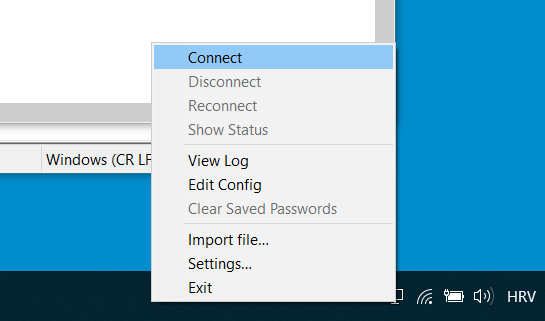
\includegraphics[width=0.5\textwidth]{OVPN-win/slika15}
     \caption{Povezivanje sa serverom}
     \label{fig:povezivanje-open}
\end{figure}
\FloatBarrier 	
Pokrenut bi server trebao izgledati kao na slici \ref{fig:status-open}.
\begin{figure}[h!]
	\centering
     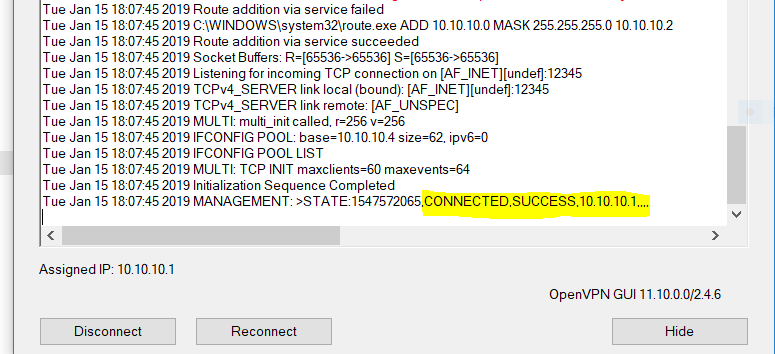
\includegraphics[width=0.7\textwidth]{OVPN-win/slika16}
     \caption{Status servera}
     \label{fig:status-open}
\end{figure}
\FloatBarrier
\newpage
\paragraph*{Konfiguracija OpenVPN klijenta}
\hfill \bigbreak

Kao prvi korak potrebno je instalirati OpenVPN kao i za server sa adrese:\smallbreak

\url{https://openvpn.net/community-downloads/}\smallbreak

Prilikom instalacije nije potrebno odabrati dodatne mogućnosti.\smallbreak
Na klijentskom računalu stvorite datoteku ``Klijent.ovpn" i kopirajte ju u 

\small\textcolor{blue}{C:\textbackslash Program Files\textbackslash OpenVPN\textbackslash easy-rsa\textbackslash keys}

\begin{figure}[h!]
	\centering
     
\includegraphics[width=0.2\textwidth]{OVPN-win/korak1}
     \caption{Prikaz Klijent.ovpn datoteke}
\end{figure}
\FloatBarrier

Konfiguracijska datoteka treba sadržavati:\smallbreak
{\small\fontfamily{pcr}\selectfont
remote 161.53.63.204\hfill;javna IP adresa računala sa serverom

client\hfill;ime uloge u mreži

port 12345\hfill;broj vrata veze

proto tcp4-client\hfill;protokol prijenosa

dev tun\hfill;stvara se virtualni tunel

tls-client\hfill;za autentifikaciju

tls-auth "C:\textbackslash \textbackslash Program Files\textbackslash \textbackslash OpenVPN\textbackslash \textbackslash easy-rsa\textbackslash \textbackslash keys\textbackslash \textbackslash ta.key" 1\hfill

; put do datoteke ključa(ta.key) te broj 1 koja označava klijenta

remote-cert-tls server

tun-mtu 1500\hfill;veličina MTU paketa

tun-mtu-extra 32\hfill;veličina MTU paketa

mssfix 1450\hfill;veličina MTU paketa

ca "C:\textbackslash \textbackslash Program Files\textbackslash \textbackslash OpenVPN\textbackslash \textbackslash easy-rsa\textbackslash \textbackslash keys\textbackslash \textbackslash ca.crt"\hfill

; put do datoteke ca.crt

cert "C:\textbackslash \textbackslash Program Files\textbackslash \textbackslash OpenVPN\textbackslash \textbackslash easy-rsa\textbackslash \textbackslash keys\textbackslash \textbackslash KlijentVPN.crt"\hfill

; put do certifikata klijenta

key "C:\textbackslash \textbackslash Program Files\textbackslash \textbackslash OpenVPN\textbackslash \textbackslash easy-rsa\textbackslash \textbackslash keys\textbackslash \textbackslash KlijentVPN.key"\hfill

; put do ključa klijenta

cipher AES-128-CBC\hfill; vrsta šifriranja

comp-lzo\hfill; kompresija podataka u tunelu

persist-key\hfill;za slučaj prekida veze

persist-tun\hfill;za slučaj prekida veze

verb 3\hfill;stupanj ispisa grešaka i upozorenja

}\bigbreak

Za upute i pojašnjenja kako odabrati ispravne vlastite parametre za ovu datoteku molimo pogledajte detaljnije upute na adresi:\smallbreak \url{https://openvpn.net/community-resources/how-to/\#config}\smallbreak

Osim toga potrebno je:
\begin{itemize}
	\item imati stabilnu vezu na internet
	\item imati omogućenu razmjenu TCP paketa u firewallu
\end{itemize}	

\paragraph*{Povezivanje klijenta i servera}
\hfill \bigbreak
Kako bi se klijent uspješno povezao na server, iz instalacijskog direktorija SERVERA kopirajte sljedeće datoteke u novu mapu koju ćete prebaciti na računala klijenata:\smallbreak
{\small\fontfamily{pcr}\selectfont
ta.key

KlijentVPN.key

KlijentVPN.csr

KlijentVPN.crt

ca.crt
}\smallbreak
Prebaciti željenim načinom na klijentsko računalo ili računala koja će se povezivati na server i kopirati u instalacijski direktorij na adresi:\smallbreak
\small\textcolor{blue}{C:\textbackslash Program Files\textbackslash OpenVPN\textbackslash easy-rsa\textbackslash keys}
\smallbreak
Ako je konfiguracija dobro odrađena, moguće je povezivanje na server. Povezivanje se započinje pokretanjem ``OpenVPN GUI'' datoteke na radnoj površini, odabirom ikone računala s alatne trake i odabirom ``Connect'' mogućnosti.
\bigbreak
Na nekim verzijama operacijskih sustava Windows potrebno je dodatno omogućiti povezivanje na interne adrese servera(npr. kao što smo postavili na 10.10.10.5) na sljedeći način:
\begin{enumerate}
  \item U tražilicu računala upisati \small\textcolor{blue}{regedit}
  \item Pozicionirati se na lokaciju s adresom \small\textcolor{blue}{Computer\textbackslash HKEY\_LOCAL\_MACHINE\newline
  \textbackslash SYSTEM\textbackslash CurrentControlSet\textbackslash Services\textbackslash Tcpip\textbackslash Parameters}
  \item Pronaći IPEnableRouter te postaviti vrijednost na 1 i na računalu servera i na računalu klijenta
\end{enumerate}
\bigbreak

Prilikom komplikacija ili nejasnoća pogledati detaljnije upute na adresi:\smallbreak
\url{https://openvpn.net/community-resources/how-to/\#config}
\smallbreak
	
	\newpage
	\subsection{FreeBSD}
	\subsubsection{OpenVPN}
	Ovo poglavlje će uključivati postavljanje VPN-a na FreeBSD inačici operacijskog
sustava BSD. 
    Potreban nam je poslužitelj za po mogućnosti sa statičkom IP adresom. Ovdje
    ćemo koristiti platformu DigitalOcean koja omogućuje brzo i jednostavno
    podizanje i upravljanje poslužiteljem. Za pristup poslužitelju koristit ćemo
    ssh protokol za što nam je potreban par ključeva koje generiramo naredbom \\

    \noindent
    \code{\$ ssh-keygen -t rsa -b 2048} \\

    \noindent
    Javni ključ se nalazi u datoteci \code{~/.ssh/id\_rsa.pub}, a privatni, koji
    mora ostati tajan, u \code{~/.ssh/id\_rsa}.

    Nakon registracije na Digital Ocean na svojem profilu možemo dodati javni ključ
    koji ćemo kasnije koristiti za pristup poslužitelju. Sada možemo stvoriti
    poslužitelja. Odabrat ćemo opciju
    \textit{Create Droplet} i odabrati sljedeće postavke:

    \begin{figure}[h]
        \centering
        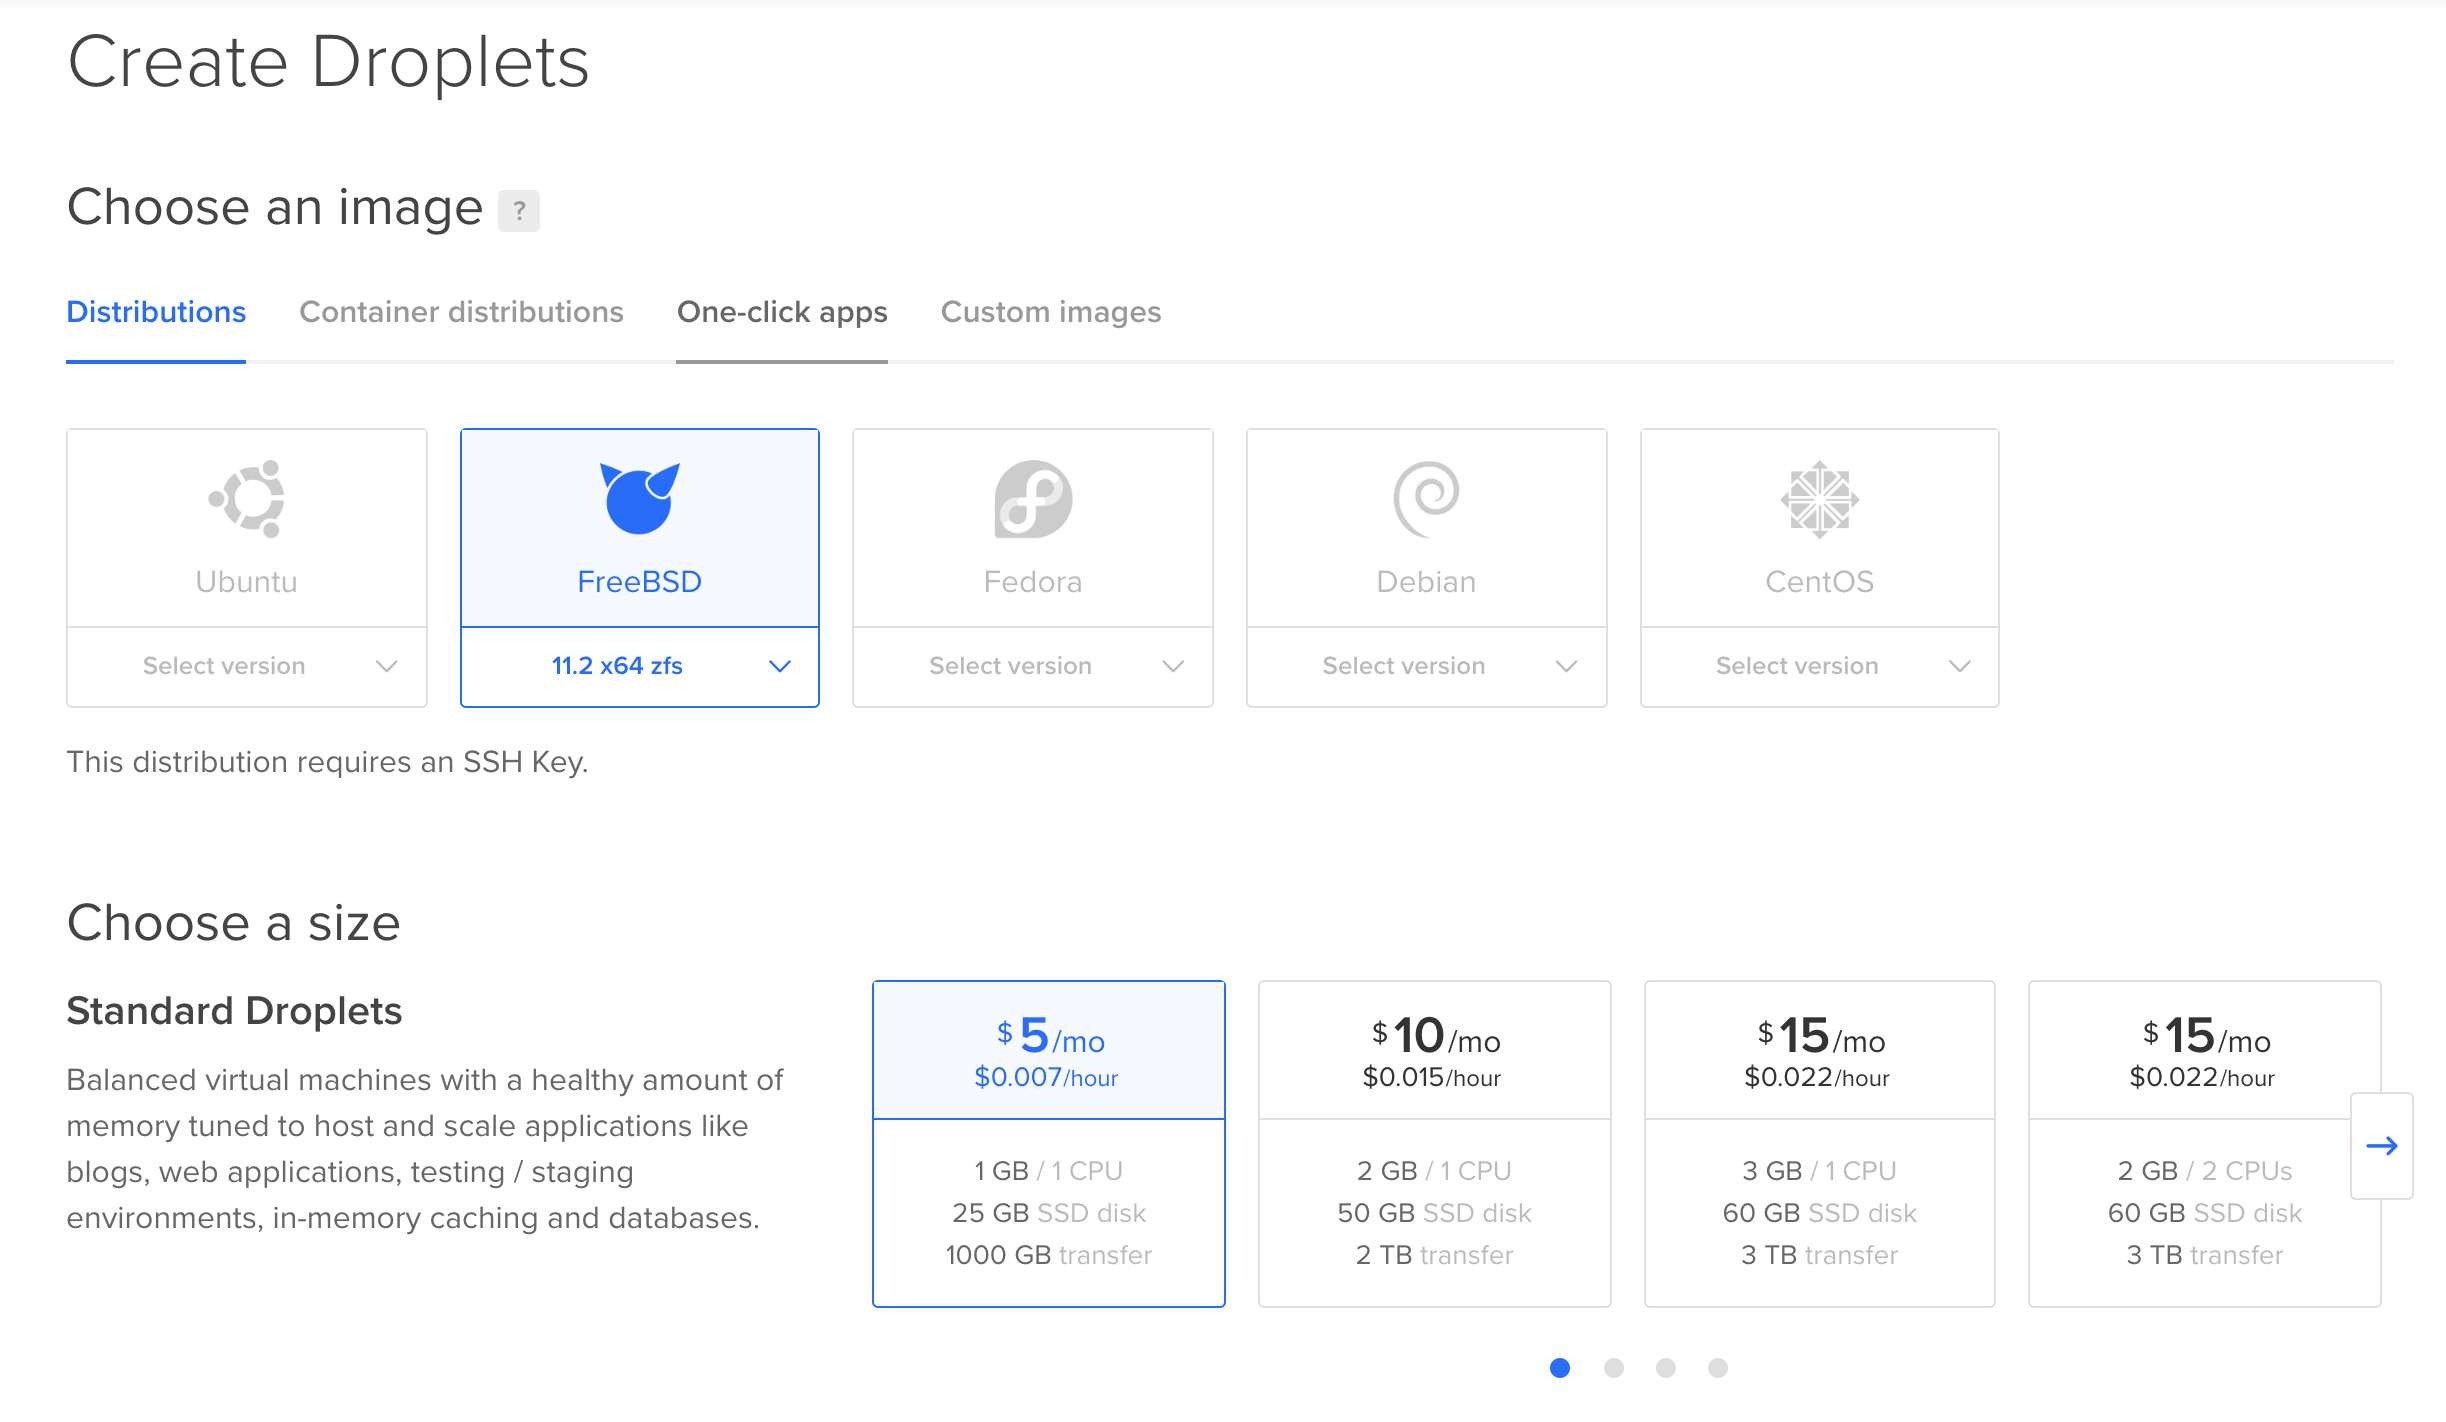
\includegraphics[scale=0.35]{slike/postavkeDOserver}
        \caption{Postavke DigitalOcean poslužitelja}
    \end{figure}

    \newpage
    \noindent
    Digital Ocean nam također nudi opciju da odaberemo lokaciju našeg poslužitelja
    i pripremimo ssh ključeve kako bi si olakšali pristup
    \begin{figure}[h]
        \centering
        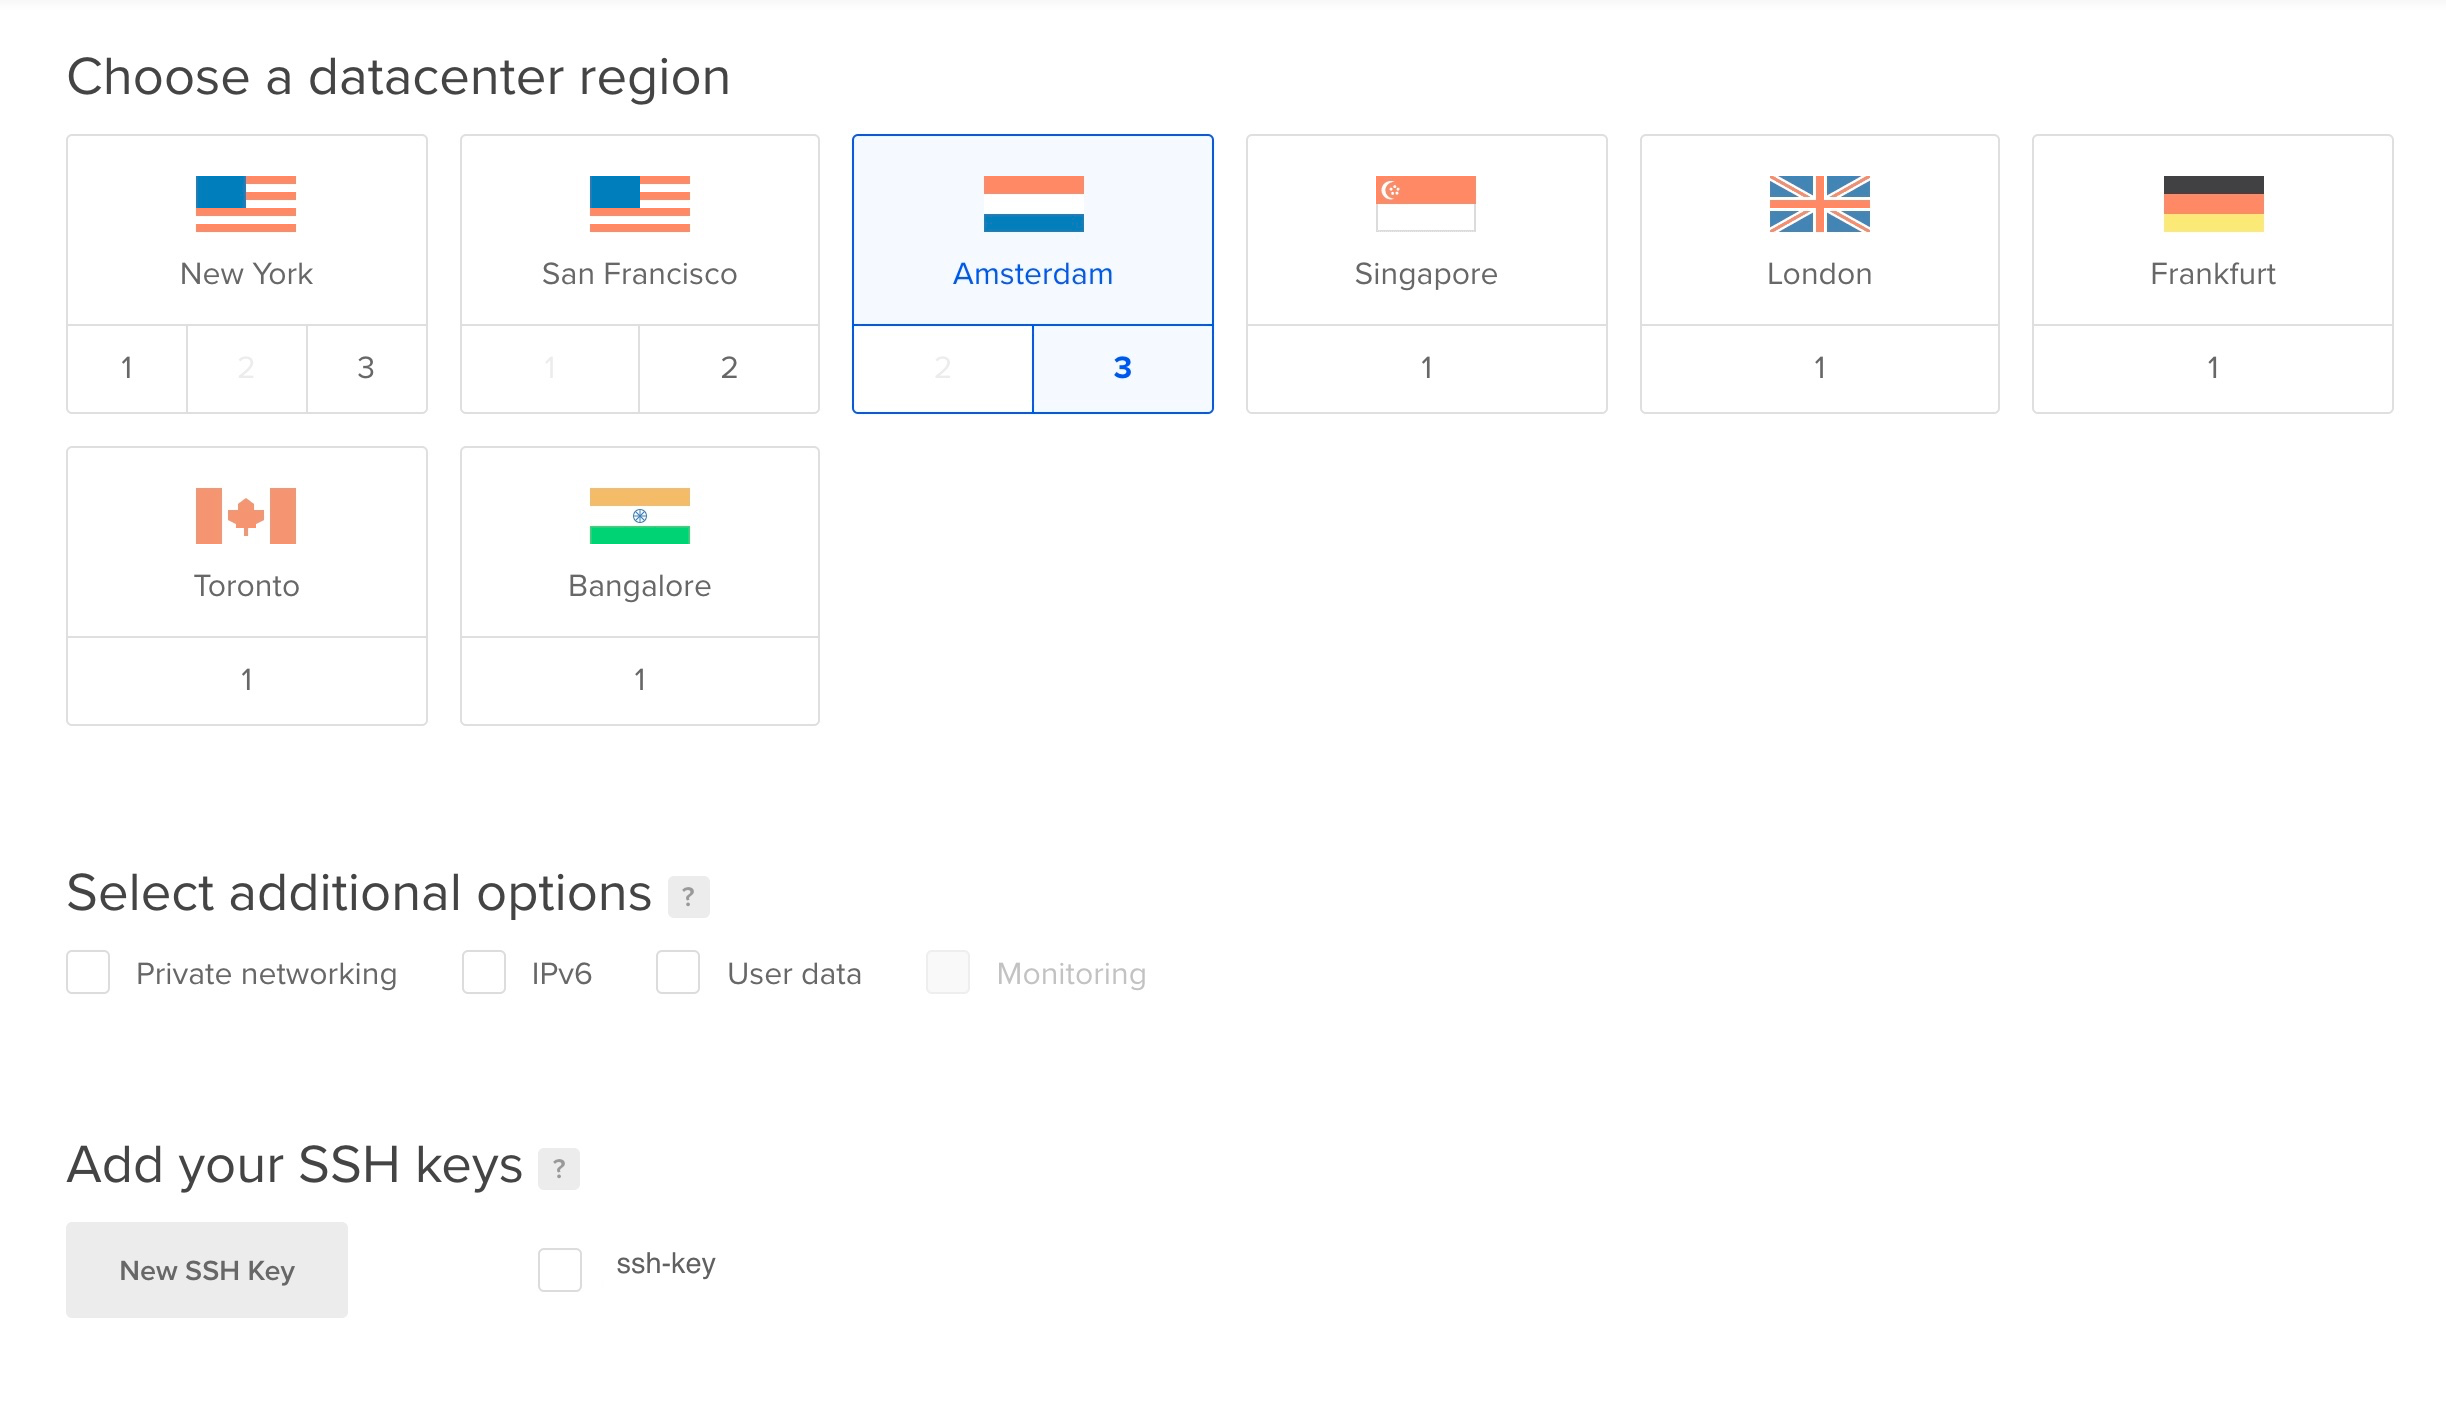
\includegraphics[scale=0.15]{slike/lokacijaIssh}
        \caption{Odabir lokacije i ssh ključeva}
    \end{figure}

    Kako sada prvi puta pristupamo poslužitelju jedini korisnik
    koji postoji je root. Root je korisnik na unixoidima koji može izvršiti
    svaku naredbu i pristupiti svakoj datoteci. Njemu pristupamo naredbom \\
    
    \noindent
    \code{\$ ssh root@139.59.159.111} \\

    Kada smo se prijavili na poslužitelja prvu stvar koju moramo napraviti je
    ažurirati sustav. To ćemo napraviti koristeći FreeBSD-ov upravitelj
    paketima \code{pkg} i njegove naredbe \code{update} i \code{upgrade}. \\

    \noindent
    \code{\# pkg update} \\
    \code{\# pkg upgrade} \\

    Sada možemo instalirati OpenVPN. \\

    \noindent
    \code{\# pkg install openvpn} \\

    Konfiguracijske datoteke ćemo smjestiti u direktorij
    \code{/usr/local/etc/openvpn} koji prvo moramo stvoriti. \\

    \noindent
    \code{\# mkdir /usr/local/etc/openvpn} \\

    \noindent
    Openvpn nudi predloške konfiguracijskih datoteka stoga ćemo kopirati
    predložak za konfiguraciju poslužitelja u naš direktorij

    \noindent
    \code{\# cp
    /usr/local/share/examples/openvpn/sample-config-files/server.conf
    \textbackslash} \\
    \code{\-\ \-\ \-\ \-\ \-\ /usr/local/etc/openvpn/openvpn.conf}

        Kako bi mogli zaštititi našu vezu potrebno je šifrirati sav promet
        između poslužitelja i klijenta i osigurati integritet svake poruke.
        Za šifriranje podataka ćemo koristiti simetrično šifriranje zbog svoje
        brzine, a za to nam je potreban simetrični ključ odnosno više ukoliko
        netko uspije dešifrirati jednu od naših poruka. Kako bi osigurali
        integritet poruka potrebno ih je potpisati i omogućiti provjeru
        potpisa. Ovaj problem ćemo riješiti digitalnim certifikatima koje ćemo
        sami napraviti. OpenVPN dolazi s alatom Easy-RSA koji će nam poslužiti za izgradnju
        infrastrukture javnog ključa (\textit{engl. PKI - public key
        infrastructure}). PKI služi kako bi se javni ključevi povezali s
        pripadajućim osobama ili organizacijama. Proces povezivanja izvršava
        tijelo za certificiranje (\textit{engl. CA - certification authority}.
        CA također potvrđuje pripada li javni ključ osobi navedenoj u
        certifikatu. U praksi se CA nalazi na posebnom računalu, ali kako ovo
        radimo za privatnu uporabu naš CA će se nalaziti na poslužitelju.

        Kako je Easy-RSA omotač oko složene programske knjižnice OpenSSL ona
        nam je jedini preduvjet te ćemo ju instalirati naredbom \\

        \noindent
        \code{\# pkg install openssl} \\

        Nakon toga ćemo kopirati \code{easy-rsa} direktorij u naš direktorij sa svom
        konfiguracijom. \\

        \noindent
        \code{\# cp -r /usr/local/share/easy-rsa
        /usr/local/etc/openvpn/easy-rsa} \\

        Sada ćemo se premjestiti u Easy-RSA direktoriji i urediti njegovu
        konfiguracijsku datoteku \code{vars}. \\

        \noindent
        \code{\# cd /usr/local/etc/openvpn/easy-rsa} \\
        \code{\# vim vars} \\

        U nastavku su navedena polja koja je potrebno izmijeniti:
        
        \noindent
        \code{set\_var EASYRSA\_REQ\_COUNTRY   \-\ "<ZEMLJA>"} \\
        \code{set\_var EASYRSA\_REQ\_PROVINCE  "<ZUPANIJA>"} \\
        \code{set\_var EASYRSA\_REQ\_CITY      \-\ \-\ \-\ \-\ "<GRAD>"} \\
        \code{set\_var EASYRSA\_REQ\_ORG       \-\ \-\ \-\ \-\ \-\ "<ORGANIZACIJA>"} \\
        \code{set\_var EASYRSA\_REQ\_EMAIL     \-\ \-\ \-\ "<EMAIL>"} \\
        \code{set\_var EASYRSA\_REQ\_OU        \-\ \-\ \-\ \-\ \-\ \-\  "<ORGANIZACIJSKA JEDINICA>"} \\
        \code{set\_var EASYRSA\_KEY\_SIZE      \-\ \-\ \-\ \-\ <broj> \# duljina rsa ključa u
        bitovima} \\
        \code{set\_var EASYRSA\_CA\_EXPIRE     \-\ \-\ \-\ <broj> \# trajanje CA ključa u
        danima} \\
        \code{set\_var EASYRSA\_CERT\_EXPIRE   \-\ <broj> \# trajanje certifikata u
        danima} \\

        Kako je \code{easy-rsa} skripta pisana za ljusku sh, dok
        FreeBSD koristi csh potrebno je naredbom \code{sh} 
        pokrenuti sh ljusku. Sada možemo inicijalizirati PKI \\

        \code{\# ./easy-rsa.real init-pki} \\
        
        \begin{figure}[H]
            \centering
            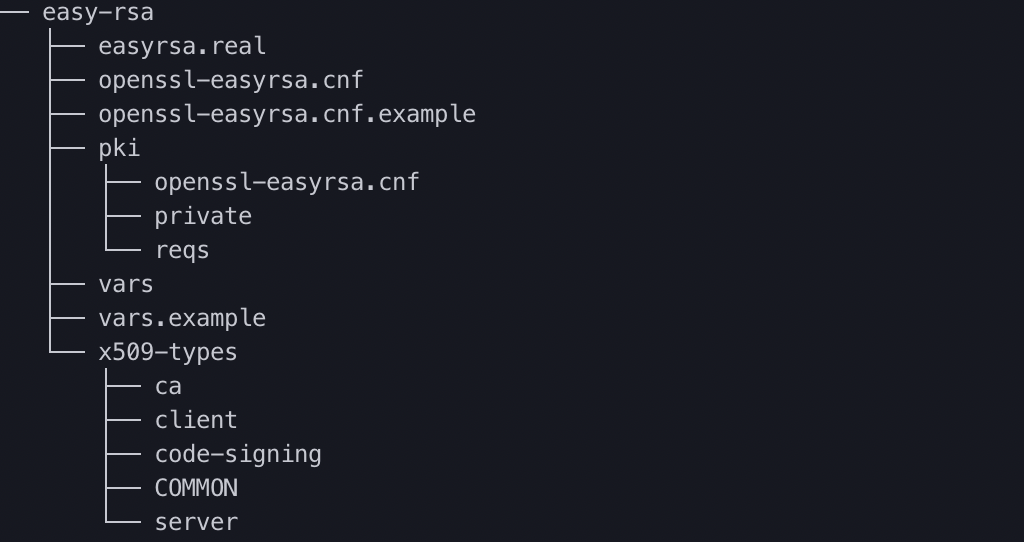
\includegraphics[scale=0.5]{slike/afterPkiInit}
            \caption{Struktura direktorija nakon inicijalizacije PKI}
        \end{figure}
        
        \noindent
        nakon čega ćemo stvoriti CA  \\

        \noindent
        \code{\# ./easy-rsa.real build-ca} \\
        
        \begin{figure}[H]
            \centering
            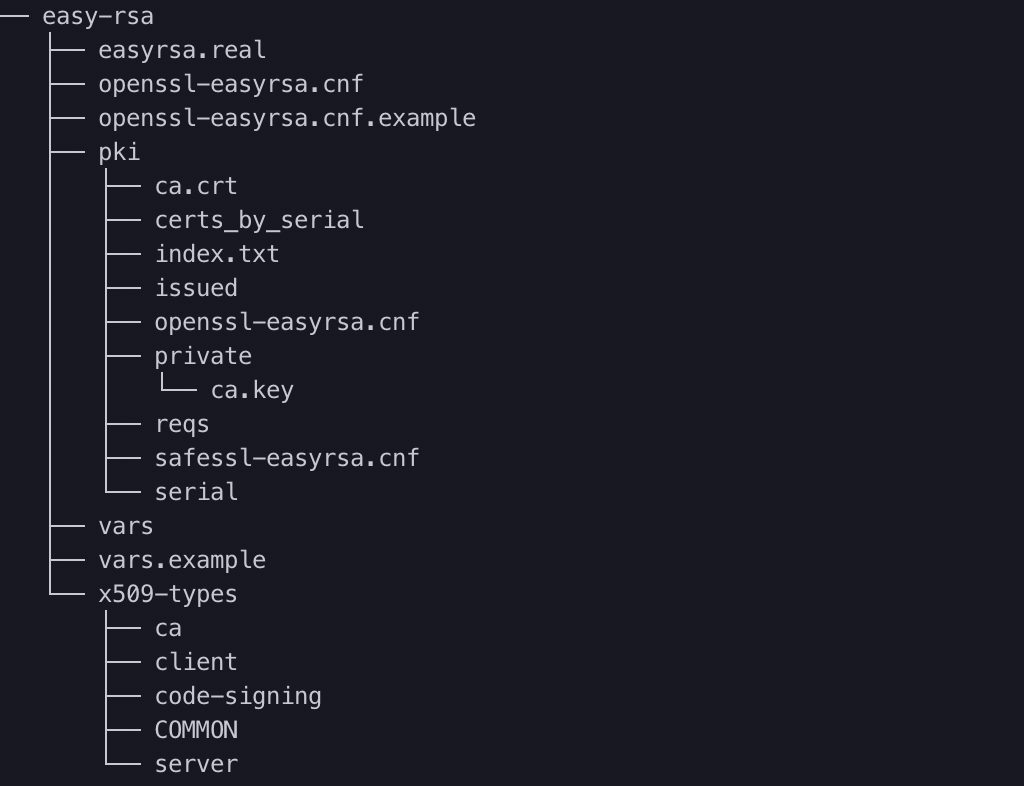
\includegraphics[scale=0.5]{slike/afterBuildCa}
            \caption{Struktura direktorija nakon stvaranja korijenskog
            certifikata}
        \end{figure}

        \noindent
        Ovom naredbom smo stvorili par ključeva koji ćemo koristiti za
        potpisivanje izdanih certifikata. 

        \noindent
        Sada ćemo generirati serverov certifikat naredbom \\

        \noindent
        \code{\# ./easy-rsa.real build-server-full <ime-server> nopass } \\

        \noindent
        gdje je \code{<ime-server>} ime certifikata, a s \code{nopass} opcijom ćemo
        generirati nešifrirani ključ kako bi mogli automatski pokrenuti OpenVPN
        uslugu prilikom pokretanja sustava bez upisivanja lozinke ključa.

        Na sličan način ćemo generirati klijentove certifikate \\

        \noindent
        \code{\# ./easy-rsa.real build-client-full <ime-klijent> nopass} \\
        
        \begin{figure}[H]
            \centering
            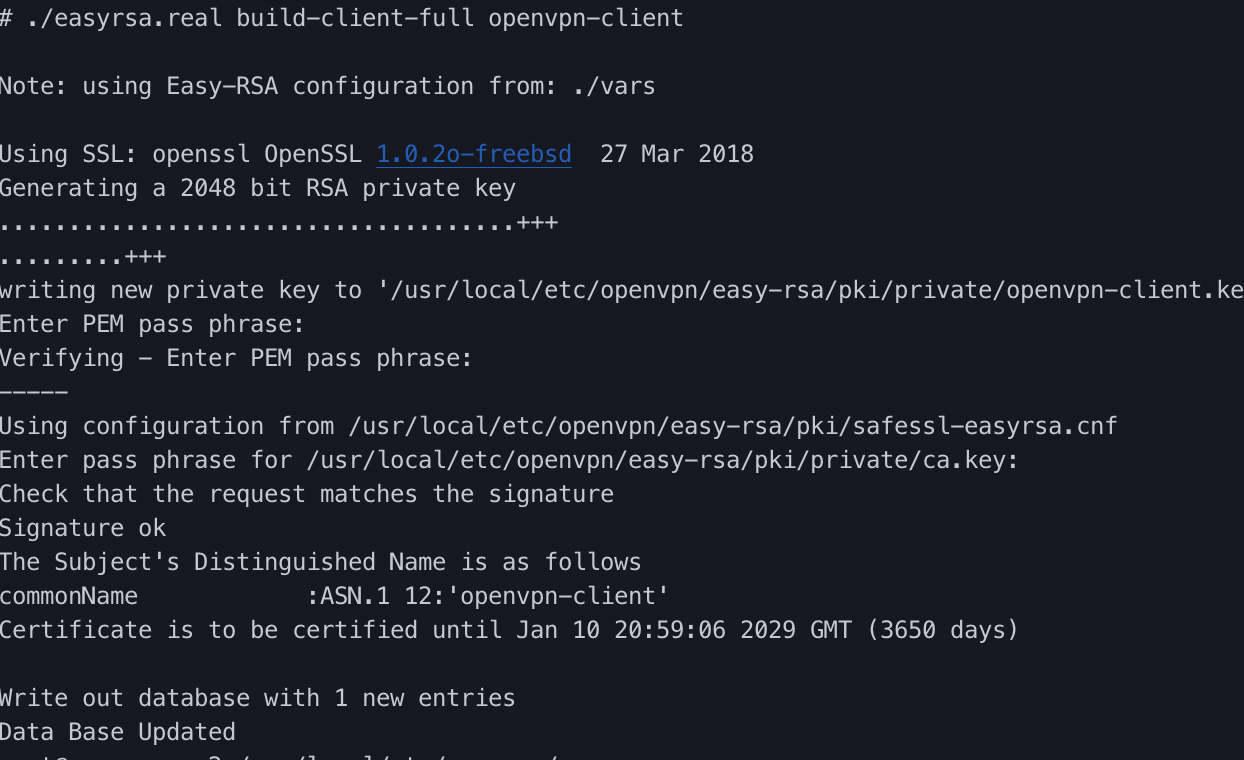
\includegraphics[scale=0.5]{slike/buildClientCert}
            \caption{Stvaranje certifikata}
        \end{figure}

        \begin{figure}[H]
            \centering
            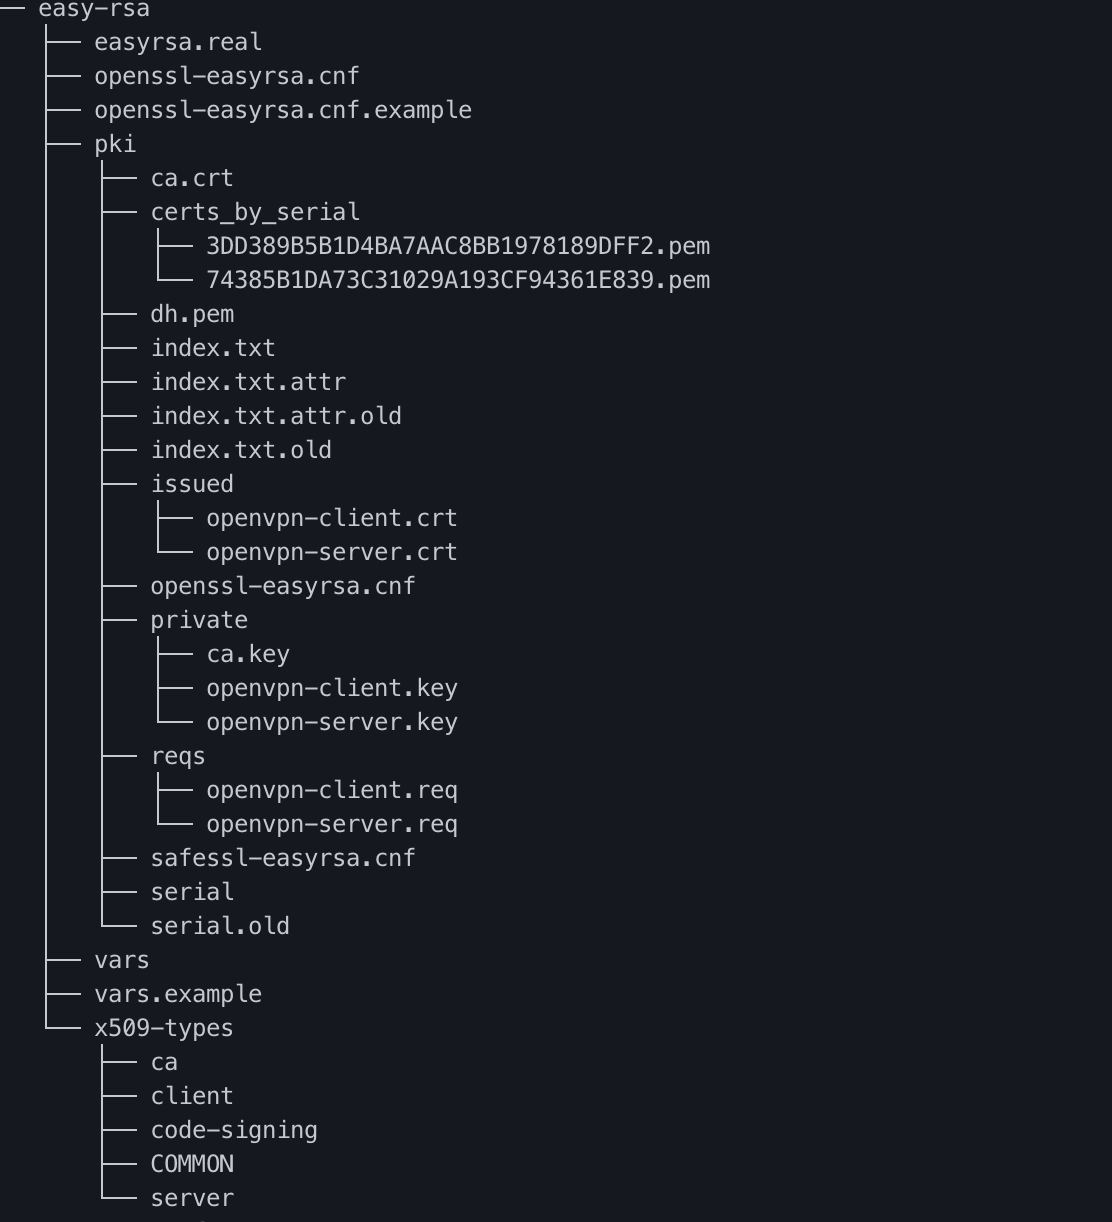
\includegraphics[scale=0.5]{slike/afterClientAndServerCert}
            \caption{Struktura direktorija nakon stvaranja klijentskog i
            poslužiteljevog certifikata}
        \end{figure}

        \noindent
        Za šifriranje same poruke koristit ćemo simetričan ključ generiran
        Diffie-Hellman razmjenom. Za to su nam potrebni Diffie-Hellman
        parametri koje stvaramo naredbom \\

        \noindent
        \code{\# ./easyrsa.real gen-dh} \\


        \noindent
        Do sada smo sve naredbe izvršavali na poslužitelju te smo generirali
        velik broj datoteka od kojih ćemo neke morati premjestiti na klijentsko
        računalo. Kako bi znali koje datoteke premjestiti potrebno je razumjeti
        čemu svaka od njih služi. Sve su datoteke stvorene u
        \code{easy-rsa/pki/} 
        direktoriju pa ćemo se u njega pozicionirati. \\

        \begin{itemize}
        \item \code{ca.crt} - certifikat koji se koristi za validaciju ostalih
        certifikata, potrebno ga je kopirati na poslužitelja i sve klijente
        \item \code{ca.key} - ključ koji CA koristi za izdavanje certifikata
        \item \code{reqs/} - direktorij koji sadrži zahtjeve za izdajom
        certifikata 
        \item \code{issued/<ime-server>.crt} - certifikat servera koji služi za
        provjeru potpisa na poruci, potrebno ga je prebaciti na poslužitelja
        \item \code{private/<ime-server>.key} - privatni ključ poslužitelja
        koji se koristi za potpisivanje poruke, potrebno ga je prebaciti na
        poslužitelja
        \item \code{issued/<ime-klijent>.crt} - certifikat klijenta koji služi za
        provjeru potpisa na poruci, potrebno ga je prebaciti na klijentsko
        računalo
        \item \code{private/<ime-klijent>.key} - privatni ključ klijenta
        koji se koristi za potpisivanje poruke, potrebno ga je prebaciti na
        klijentsko računalo
        \item \code{dh.pem} - Diffie Hellman parametri, potrebno ih je prebaciti na
        poslužitelja
        \end{itemize}

        \noindent
        Ključeve poslužitelja ćemo premjestiti u poseban direktorij \\

        \noindent
        \code{\# mkdir /usr/local/etc/openvpn/keys} \\
        \code{\# cp pki/dh.pem \textbackslash} \\
        \code{\-\ \-\ \-\ \-\ \-\ pki/ca.crt \textbackslash} \\
        \code{\-\ \-\ \-\ \-\ \-\ pki/issued/<ime-server>.crt \textbackslash} \\
        \code{\-\ \-\ \-\ \-\ \-\ pki/private/<ime-server>.key \textbackslash} \\
        \code{\-\ \-\ \-\ \-\ \-\ /usr/local/etc/openvpn/keys} \\

        \begin{figure}[H]
            \centering
            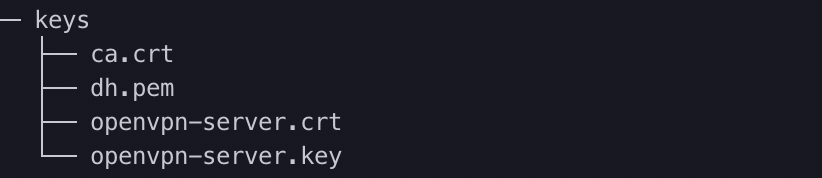
\includegraphics[scale=0.7]{slike/serverKeys}
            \caption{Sadržaj \code{keys} direktorija na poslužitelju}
        \end{figure}

        \noindent
        Prije nego što počnemo konfigurirati klijentsko računalo, potrebno je u
        konfiguraciji poslužitelja navesti putanje do certifikata, ključeva i 
        parametara. To ćemo napraviti u datoteci \code{openvpn.conf} koju smo
        na samom početku kopirali u \code{/usr/local/etc/openvpn}. \\
        
        \noindent
        \code{\# vim /usr/local/etc/openvpn/openvpn.conf} \\
        
        \noindent
        Potrebno je urediti sljedeće linije \\

        \noindent
        \code{ca /usr/local/etc/openvpn/keys/ca.crt} \\
        \code{cert /usr/local/etc/openvpn/keys/<ime-server>.crt} \\
        \code{key /usr/local/etc/openvpn/keys/<ime-server>.key} \\
        \code{dh /usr/local/etc/openvpn/keys/dh.pem} \\ 

        \begin{figure}[H]
            \centering
            \includegraphics[scale=0.57]{slike/serverPaths}
            \caption{Putanje do ključeva i certifikata u datoteci
            \code{openvpn.conf}}
        \end{figure}
        
        Sada možemo postaviti klijentsko računalo. Kako smo već pripremili
        većinu klijentovih datoteka na poslužitelju, potrebno ih je kopirati.
        Radi se o osjetljivim datotekama stoga nam je potreban siguran način
        slanja datoteka preko mreže za što ćemo koristiti program
        \textit{secure copy}. Nakon što instaliramo openvpn isto kao i na
        poslužiteljskom računalu možemo kopirati predložak konfiguracije \\

        \noindent
        \code{\# cp
        /usr/local/share/examles/openvpn/sample-config-files/client.config
        \textbackslash} \\
        \code{\-\ \-\ \-\ \-\ \-\ /usr/local/etc/openvpn/openvpn.conf} \\

        \noindent
        Također stvorit ćemo direktorij u koji ćemo spremiti ključeve i
        certifikate \\

        \noindent
        \code{\# mkdir /usr/local/etc/openvpn/keys}\\

        \noindent
        Sada možemo kopirati potrebne datoteke s poslužitelja \\

        \noindent
        \code{\$ scp
        root@<ip-server>:/usr/local/etc/openvpn/easy-rsa/pki/ca.crt keys } \\
        \code{\$ scp
        root@<ip-server>:\textbackslash} \\
        \code{\-\
        \-\ \-\ \-\ \-\ \-\ /usr/local/etc/openvpn/easy-rsa/pki/issued/<ime-klijent>.crt
        \textbackslash} \\
        \code{\-\ \-\ \-\ \-\ \-\ \-\ keys} \\
        \code{\$ scp
        root@<ip-server>:\textbackslash} \\
        \code{\-\
        \-\ \-\ \-\ \-\ \-\
        /usr/local/etc/openvpn/easy-rsa/pki/private/<ime-klijent>.key
        \textbackslash} \\
        \code{\-\ \-\ \-\ \-\ \-\ \-\ keys} \\

        \begin{figure}[H]
            \centering
            \includegraphics[scale=0.7]{slike/clientKeys}
            \caption{Sadržaj \code{keys} direktorija na klijentu}
        \end{figure}

        \noindent
        U konfiguraciji (\code{openvpn.conf}) osim putanja do certifikata i
        ključeva potrebno je unijeti ip adresu poslužitelja \\

        \noindent
        \code{remote <ip-server> 1194} \\
        \code{ca /usr/local/etc/openvpn/keys/ca.crt} \\
        \code{cert /usr/local/etc/openvpn/keys/<ime-server>.crt} \\
        \code{key /usr/local/etc/openvpn/keys/<ime-server>.key} \\

        Za upravljanje servisima koristimo naredbu \code{service}. Prvo ćemo
        njome pokrenuti OpenVPN servis na poslužitelju i nakon toga na klijentu

        \noindent
        \code{\# service openvpn run} \\

        \noindent
        Sada možemo alatom \code{ifconfig} provjeriti stanje mrežnih sučelja \\
        na klijentu: \\
        \begin{figure}[H]
            \centering
            \includegraphics[scale=0.5]{slike/clientIfconfig}
            \caption{Mrežna sučelja klijenta }
        \end{figure}
        na poslužitelju: \\
        \begin{figure}[H]
            \centering
            \includegraphics[scale=0.5]{slike/serverIfconfig}
            \caption{Mrežna sučelja poslužitelja}
        \end{figure}

        Možemo uočiti novo sučelje \code{tun0} koje predstavlja virtualno
        sučelje mrežnog sloja. Izvršavanjem naredbe \code{ping} možemo provjeriti je
        li klijentsko računalo stvarno povezano s poslužiteljem. \\

        \noindent
        \code{\$ ping 10.8.0.1} \\

        Kako nam je cilj povezati dva klijenta koji se nalaze u različitim
        privatnim mrežama na isti ćemo pripremiti još jednog klijenta. Njegova
        konfiguracija će biti jednaka konfiguraciji prvog klijenta, a izlaz
        naredbe \code{ifconfig}:
        \begin{figure}[H]
            \centering
            \includegraphics[scale=0.45]{slike/client2Ifconfig}
            \caption{Mrežna sučelja drugog klijenta}
        \end{figure}

        \noindent
        Ako sada pokušamo naredbom
        \code{\$ ping 10.8.0.6}
        provjeriti jesu li klijenti međusobno povezani nećemo dobiti nikakav
        rezultat. Razlog tome je što pretpostavljena konfiguracija poslužitelja
        ne dozvoljava komunikaciju između klijenata. Kako bi to omogućili
        potrebno je u konfiguracijskoj datoteci poslužitelja otkomentirati liniju 

        \noindent 
        \code{client-to-client} \\

        \noindent
        Sada ćemo ponovo pokrenuti OpenVPN i ispitati jesu li klijenti
        međusobno povezani \\

        \noindent
        \code{\# service openvpn restart} \\
        \code{\$ ping 10.8.0.6} \\
        \begin{figure}[H]
            \centering
            \includegraphics[scale=0.5]{slike/pingResult}
            \caption{Izlaz naredbe ping}
        \end{figure}

        Za kraj možemo pokušati kopirati datoteku s jednog klijenta na drugi
        koristeći \code{tun0} sučelja. Na klijentu s adresom \code{10.8.0.6}
        stvorit ćemo datoteku \code{pozdrav.txt} i u nju nešto zapisati \\ 

        \noindent
        \code{\$ touch pozdrav.txt} \\
        \code{\$ echo "Bok" > pozdrav.txt} \\

        \noindent
        Sada ćemo s drugog klijenta (adresa \code{10.8.0.10}) kopirati
        \code{pozdrav.txt} datoteku i ispisati ju \\
        \code{\$ scp root@10.8.0.6:/root/pozdrav.txt .} \\
        \code{\$ cat /root/pozdrav.txt}\\

        \begin{figure}[H]
            \centering
            \includegraphics[scale=0.45]{slike/pozdrav}
            \caption{Kopiranje i ispis datoteke \code{pozdrav.txt}}
        \end{figure}


	\newpage
	\subsection{Linux}
	 Linux distribucije podržavaju mnogobrojni VPN-ovi. U sljedećim poglavljima bit će opisana instalacija dva različita VPN-a na Ubuntu distribuciju Linux operacijskog sustava. Upute za OpenVPN su složenije i namijenjene su naprednijim korisnicima, dok upute za LibreSwan koriste već unaprijed napisanu skriptu i prilagođene su korisnicima koji su početnici ili žele što brže uspostaviti VPN, a uz što manje truda.
	\subsubsection{OpenVPN}
	

\lstset{
	escapeinside={(*@}{@*)}
}

\bigbreak
\paragraph*{Što je OpenVPN?}
\hfill \smallbreak
OpenVPN\cite{openvpn} je potpuno otvoreni kod za SSL VPN soluciju koji zastupa širok raspon različitih konfiguracija, pritom uključujući udaljeni pristup, \textit{site-to-site} VPN-ove, sigurnost Wi-Fi-a te nudi rješenja za udaljeni pristup prilagođen profesionalnim okruženjima. Sigurnosni model OpenVPN-a bazira se na protokolima SSL/TLS, koji su industrijski standard za sigurnu komunikaciju preko interneta.

\bigbreak
\paragraph*{Prije početka instalacije}
\hfill \smallbreak
 Ove upute\cite{tutorialopenvpn} prilagođene su za verziju 16.04 Ubuntu distribucije operacijskog sustava Linux. Za uspješno instaliranje OpenVPN-a potrebna vam je javna IP adresa te je istu potrebno doznati prije početka instalacije. To se može doznati klikom na sljedeću stranicu \url{https://www.whatismyip.com/ }. Isto tako potrebno je otvoriti određena vrata (eng. \textit{port}) na vašem usmjeritelju ili ako je to zabranjeno od vašeg pružatelja internetskih usluga onda možete računalo potpuno izložiti internetu tako da se u postavkama usmjeritelja podesi opcija DMZ Host na IP adresu vašeg računala (ovaj način se ne preporuča jer vašu lokalnu mrežu izlaže internetu što predstavlja sigurnosni problem).
 \\
 Sljedeći koraci izvedeni su u Ubuntu v. 16.04 u virtualnom okruženju.
 
 \bigbreak
 \paragraph*{Instalacija OpenVPN-a}
 \hfill \smallbreak
 Prvi korak je instalacija OpenVPN-a te paketa easy-rsa (koji će poslužiti kao naše privatno lokalno certifikacijsko tijelo) na naš operacijski sustav. \\
 Počnimo prvo s osvježavanjem sustava te instalacijom nužnih paketa:
\begin{lstlisting}
 sudo apt-get update
 sudo apt-get install openvpn easy-rsa
\end{lstlisting}
 Sljedeći korak je uspostava certifikacijskog tijela. Kopirat ćemo easy-rsa predložak u novi direktorij te se nakon toga pozicionirati u njega:
\begin{lstlisting}
 make-cadir (*@$\sim$@*)/openvpn-ca
 cd (*@$\sim$@*)/openvpn-ca
\end{lstlisting}
Konfigurirajmo sada vrijednosti koje će naše tijelo koristiti otvaranjem datoteke vars:
\begin{lstlisting}
 nano vars
\end{lstlisting}
Unutra se nalaze neke varijable koje definiraju način stvaranja certifikata. Nas zanimaju samo neke od njih. Plave vrijednosti postavite po želji, a ako za KEY NAME koristite neku drugu vrijednost zapamtite ju jer će nam kasnije biti potrebna.

\begin{lstlisting}
 export KEY_COUNTRY="(*@\textcolor{blue}{HR}@*)"
 export KEY_PROVINCE="(*@\textcolor{blue}{ZG}@*)"
 export KEY_CITY="(*@\textcolor{blue}{Zagreb}@*)"
 export KEY_ORG="(*@\textcolor{blue}{FER}@*)"
 export KEY_EMAIL="(*@\textcolor{blue}{info@primjer.hr}@*)"
 export KEY_OU="(*@\textcolor{blue}{Grupa za projekt}@*)"

 export KEY_NAME="(*@\textcolor{blue}{server}@*)"
\end{lstlisting}
 Nakon što ste završili spremite i izađite. 

 \begin{figure}[h]
 	\centering
 	\includegraphics[width=0.7\linewidth]{"slike/OpenVPN/Screenshot from 2018-12-14 18-30-43"}
 	\caption[Postavljanje vrijednosti za certifikacijsko tijelo]{Postavljanje vrijednosti za CA}
 	\label{fig:screenshot-from-2018-12-14-18-30-43}
 \end{figure}
 
\bigbreak
\paragraph*{Izgradnja certifikacijskog tijela}
\hfill \smallbreak
Osigurajte da se nalazite u dobrom direktoriju i onda postavite datoteku vars kao izvor:
\begin{lstlisting}
 cd (*@$\sim$@*)/openvpn-ca
 source vars
\end{lstlisting}

\begin{figure}[h]
	\centering
	\includegraphics[width=0.7\linewidth]{"slike/OpenVPN/Screenshot from 2018-12-14 18-32-06"}
	\caption[Dobar ispis nakon postavljanja izvorišta]{Dobar ispis nakon postavljanja izvorišta}
	\label{fig:screenshot-from-2018-12-14-18-32-06}
\end{figure}


Ako je sve prošlo kako treba trebali bi imati ispis kao na slici \ref{fig:screenshot-from-2018-12-14-18-32-06} te nakon toga osigurat ćemo čisti start i krenut ćemo u izgradnju našeg tijela. Zadnja naredba će inicirati izgradnju tijela - pritisnite ENTER na već ponuđene parametre.
\begin{lstlisting}
 ./clean-all
 ./build-ca
\end{lstlisting}

\begin{figure}[h]
	\centering
	\includegraphics[width=0.7\linewidth]{"slike/OpenVPN/Screenshot from 2018-12-14 18-40-25"}
	\caption[Dogodila se pogreška prilikom izgradnje CA]{Dogodila se pogreška prilikom izgradnje CA}
	\label{fig:screenshot-from-2018-12-14-18-40-25}
\end{figure}


U slučaju pogreške, kao što je prikazano na slici \ref{fig:screenshot-from-2018-12-14-18-40-25} , unesite sljedeće naredbe:
\begin{lstlisting}
 ln -s openssl-1.0.0.cnf openssl.cnf
 ./build-ca
\end{lstlisting}
Sada bi sve trebalo biti uredu.\\

Nastavimo dalje s izradom poslužiteljskog certifikata, ključa te enkripcijskih datoteka. Prvo ćemo generirati ključ za poslužitelj. Prihvatite unaprijed određene parametre pritiskom tipke ENTER i ne unosite lozinku. Pred kraj bit će te pitani dva pitanja, na oba odgovorite sa \textbf{y}.\\
NAPOMENA: U slučaju da ste odabrali neko drugo ime, a ne server onda u sljedećim koracima svaku pojavu riječi server zamijenite s vašim imenom! 
\begin{lstlisting}
 ./build-key-server server
\end{lstlisting}
Generirat ćemo još neke dijelove poput Diffie-Hellman ključeva koji će se koristit prilikom razmjene ključeva:
\begin{lstlisting}
 ./build-dh
 openvpn --genkey --secret keys/ta.key
\end{lstlisting}

\bigbreak
\paragraph*{Generiranje klijentskog certifikata}
\hfill \smallbreak
Sljedeći korak nam je generiranje certifikata za klijenta te par ključa. Iako se ovo može izvesti na računalu klijenta zbog jednostavnosti ovdje ćemo odraditi te korake. Za ime klijenta koristit ćemo client1. Kasnije se možete vratiti na ovaj korak za generiranje ključeva za druge klijente.\\
Za izradu lozinkom ne zaštićenih podatak upišite:

\begin{lstlisting}
 cd (*@$\sim$@*)/openvpn-ca
 source vars
 ./build-key client1
\end{lstlisting}
U slučaju da želite lozinkom zaštititi:  
\begin{lstlisting}
 cd (*@$\sim$@*)/openvpn-ca
 source vars
 ./build-key-pass client1
\end{lstlisting}
Opet kao i prije prihvatite ponuđene argumente pritiskom na tipku ENTER te odgovorite na pitanja sa \textbf{y}.
\bigbreak
\paragraph*{Konfiguracija OpenVPN usluge}
\hfill \smallbreak
Pozicionirajmo se prvo u /openvpn-ca-keys te zatim kopirajmo datoteke u /etc/openvpn:
\begin{lstlisting}
 cd (*@$\sim$@*)/openvpn-ca/keys
 sudo cp ca.crt server.crt server.key ta.key dh2048.pem /etc/openvpn
\end{lstlisting}
Idući korak je kopiranje i raspakiravanje primjera konfiguracije:

\begin{lstlisting}[basicstyle=\tiny]
 gunzip -c /usr/share/doc/openvpn/examples/sample-config-files/server.conf.gz | sudo tee /etc/openvpn/server.conf
\end{lstlisting}
Sada ćemo raspakiranu konfiguraciju otvoriti:
\begin{lstlisting}
 sudo nano /etc/openvpn/server.conf
\end{lstlisting}
Nađite dio koji se odnosi na HMAC tražeći tls-auth. Otkomentirajte tu liniju tako da obrišete ; ispred linije te dodajmo liniju vezanu uz smjer ključa : 
\begin{lstlisting}
 tls-auth ta.key 0 # This file is secret
 (*@\textcolor{blue}{key-direction 0}@*)
\end{lstlisting}
Sljedeće nađite liniju vezanu uz kriptografske šifrante  te ju otkomentirajte. Ispod toga dodajte algoritam za HMAC poruke:
\begin{lstlisting}
 cipher AES-256-CBC
 (*@\textcolor{blue}{auth SHA256}@*)
\end{lstlisting}
Potom otkomentirajte i sljedeće dvije linije:
\begin{lstlisting}
 user nobody
 group nogroup
\end{lstlisting}
Sljedeći dio nije potreban, ali se preporučuje. Inače VPN konekcija nije postavljena tako da sav internet promet ide kroz nju. U slučaju da želite sav internet promet preusmjeriti kroz internet konekciju otkomentirajte liniju:
\begin{lstlisting}
 push "redirect-gateway def1 bypass-dhcp"
\end{lstlisting}
Otkomentirajte obje linije koje se odnose na dhcp:
\begin{lstlisting}
 push "dhcp-option DNS 208.67.222.222"
 push "dhcp-option DNS 208.67.220.220"
\end{lstlisting}
Neobavezno-promijenite port i protokol koji se koriste. OpenVPN koristi vrata 1194 i protokol UDP za prihvat klijentskih konekcija. U slučaju da iz nekog razloga to vam ne odgovara postavite vrata na neka druga (npr. 443):
\begin{lstlisting}
 port (*@\textcolor{blue}{443}@*)
 
 proto tcp
 ;proto udp
\end{lstlisting}
U slučaju da niste koristili ime server onda ga sad promijenite u sljedećim linijama:
\begin{lstlisting}
 cert server.crt
 key server.key
\end{lstlisting}
Spremite datoteku te izađite.
\bigbreak
\paragraph*{Prilagođavanje mrežnih postavka poslužitelja}
\hfill \smallbreak
Modificirajmo postavke otvarajući datoteku:
\begin{lstlisting}
 sudo nano /etc/sysctl.conf
\end{lstlisting}
Potražite sljedeću liniju te maknite znak \# kako bi ju otkomentirali. 
\begin{lstlisting}
 net.ipv4.ip_forward=1
\end{lstlisting}
Spremite i izađite. \\
Kako bi pročitali datoteku i namjestili vrijednosti za trenutnu sesiju upišite:
\begin{lstlisting}
 sudo sysctl -p
\end{lstlisting}
Prilagodimo sada pravila vatrozida, a za to nam treba mrežno sučelje pa iz tog razloga upisujemo:
\begin{lstlisting}
 ip route | grep default
\end{lstlisting}
Izlaz bi vam trebao sličiti na doljnji ispis. Nama je važan plavo pobojan dio:
\begin{lstlisting}
 default via 192.168.0.1 dev (*@\textcolor{blue}{enp0s3}@*)  proto dhcp  metric 600
\end{lstlisting}
Otvorimo sad konfiguracijsku datoteku:
\begin{lstlisting}
 sudo nano /etc/ufw/before.rules
\end{lstlisting}
\begin{figure}[h]
	\centering
	\includegraphics[width=0.7\linewidth]{"slike/OpenVPN/Screenshot from 2018-12-14 19-06-58"}
	\caption[Izgled konfiguracijske datoteke - UFW Firewall]{Izgled konfiguracijske datoteke - UFW Firewall}
	\label{fig:screenshot-from-2018-12-14-19-06-58}
\end{figure}
U konfiguraciju dodajmo plavo označene dijelove pritom zamijenite enp0s3 za ime mrežnog sučelja koje ste maloprije otkrili. Konačan izgled trebao bi biti kao na slici \ref{fig:screenshot-from-2018-12-14-19-06-58}.
\begin{lstlisting}
 #
 # rules.before
 #
 # Rules that should be run before the ufw command line added rules. 
 # Custom rules should be added to one of these chains:
 #   ufw-before-input
 #   ufw-before-output
 #   ufw-before-forward
 #
 
 # START OPENVPN RULES
 # NAT table rules
 (*@\textcolor{blue}{*nat}@*)
 (*@\textcolor{blue}{:POSTROUTING ACCEPT [0:0]}@*)
 # Dopusti promet od OpenVPN klijenta prema enp0s3 
 (*@\textcolor{blue}{-A POSTROUTING -s 10.8.0.0/8 -o enp0s3 -j MASQUERADE}@*)
 (*@\textcolor{blue}{COMMIT}@*)
 # END OPENVPN RULES
 
 # Don't delete these required lines, otherwise there will be errors
\end{lstlisting}
Sada trebamo reći UFW-u da automatski proslijedi pakete. Otvorimo datoteku:
\begin{lstlisting}
 sudo nano /etc/default/ufw
\end{lstlisting}
Promijenimo sljedeću liniju iz DROP u ACCEPT. Spremimo datoteku i izađimo.
\begin{lstlisting}
 DEFAULT_FORWARD_POLICY="(*@\textcolor{blue}{ACCEPT}@*)"
\end{lstlisting}
Otvorimo sada port 1194 tako da prima UDP promet. U slučaju da ste mijenjali port i/ili protokol promijenite vrijednosti u svoje. Isto tako dopustit ćemo SSH promet te ćemo onda onemogućiti pa ponovno omogućiti naša nova pravila.
\begin{lstlisting}
 sudo ufw allow 1194/udp
 sudo ufw allow OpenSSH
 sudo ufw disable
 sudo ufw enable
\end{lstlisting}
\bigbreak
\paragraph*{Omogućavanje i pokretanje OpenVPN usluge}
\hfill \smallbreak
Pokrenimo uslugu te odmah potom provjerimo je li uspješno pokrenuta. U slučaju da vam se ime razlikuje od imena server, promijenite ga.
\begin{lstlisting}
 sudo systemctl start openvpn@server
 sudo systemctl status openvpn@server
\end{lstlisting}
Ispis, ako nije došlo do greške trebao bi biti kao na slici \ref{fig:screenshot-from-2018-12-14-19-10-10}.
\begin{figure}[h]
	\centering
	\includegraphics[width=0.7\linewidth]{"slike/OpenVPN/Screenshot from 2018-12-14 19-10-10"}
	\caption[Pokrenuta usluga OpenVPN]{Pokrenuta usluga OpenVPN}
	\label{fig:screenshot-from-2018-12-14-19-10-10}
\end{figure}
Možete isto tako provjeriti je li dostupno OpenVPN sučelje tun0. Ispis bi trebao biti kao na slici \ref{fig:screenshot-from-2018-12-14-19-11-00}.
\begin{lstlisting}
 ip addr show tun0
\end{lstlisting}
\begin{figure}[h]
	\centering
	\includegraphics[width=0.7\linewidth]{"slike/OpenVPN/Screenshot from 2018-12-14 19-11-00"}
	\caption[OpenVPN sučelje tun0]{OpenVPN sučelje tun0}
	\label{fig:screenshot-from-2018-12-14-19-11-00}
\end{figure}
Konačno ako je sve prošlo kako treba omogućimo automatsko pokretanje usluge:
\begin{lstlisting}
 sudo systemctl enable openvpn@server
\end{lstlisting}
\bigbreak
\paragraph*{Izrada konfiguracijske strukture klijenta}
\hfill \smallbreak
Stvorimo novi direktorij, podesimo mu postavke te nakon toga kopirajmo primjer konfiguracije u njega.Otvorimo tu konfiguraciju kako bi ju mogli urediti:
\begin{lstlisting}
 mkdir -p (*@$\sim$@*)/client-configs/files
 chmod 700 (*@$\sim$@*)/client-configs/files
\end{lstlisting}
\begin{lstlisting}[basicstyle=\tiny]
 cp /usr/share/doc/openvpn/examples/sample-config-files/client.conf (*@$\sim$@*)/client-configs/base.conf
\end{lstlisting}
\begin{lstlisting}
 nano (*@$\sim$@*)/client-configs/base.conf
\end{lstlisting}
Nađite dio konfiguracije koji se odnosi na udaljeni pristup. Ta linija upućuje klijenta na naš server. Zamijenite plavi dio linije javnom IP adresom servera ili domenom servera te napišite port koji ste odabrali.
\begin{lstlisting}
 . . .
 # The hostname/IP and port of the server.
 # You can have multiple remote entries
 # to load balance between the servers.
 remote (*@\textcolor{blue}{88.207.10.226 1194}@*)
 . . .
\end{lstlisting}
Provjerite da je dobar protokol postavljen:
\begin{lstlisting}
 proto (*@\textcolor{blue}{udp}@*)
\end{lstlisting}
Otkomentirajte korisnika i grupu:
\begin{lstlisting}
 # Downgrade privileges after initialization (non-Windows only)
 user nobody
 group nogroup
\end{lstlisting}
Zakomentirajte sljedeće linije:
\begin{lstlisting}
 #ca ca.crt
 #cert client.crt
 #key client.key
\end{lstlisting}
Unesite šifrant koji ste unijeli u /etc/openvpn/server.conf
\begin{lstlisting}
 (*@\textcolor{blue}{cipher AES-256-CBC}@*)
 (*@\textcolor{blue}{auth SHA256}@*)
\end{lstlisting}
Negdje u dokumentu dodajte sljedeću liniju:
\begin{lstlisting}
 key-direction 1
\end{lstlisting}
Na kraju dodajte par zakomentiranih linija. Njih želimo uključiti u svaku konfiguraciju iz razloga ako klijent pristupa s Linux operativnog sustava koji u sebi ima /etc/openvpn/update-resolv-conf tada će ova skripta osvježavati DNS postavke za Linux klijente.
\begin{lstlisting}
 # script-security 2
 # up /etc/openvpn/update-resolv-conf
 # down /etc/openvpn/update-resolv-conf
\end{lstlisting}
Kreirajmo sada konfiguracijsku skriptu. Stvorite i otvorite skriptu:
\begin{lstlisting}
 nano (*@$\sim$@*)/client-configs/make_config.sh
\end{lstlisting}
Kopirajte sljedeću skriptu i spremite datoteku te potom izađite.
\begin{lstlisting}[language=bash]
 #!/bin/bash
 
 # First argument: Client identifier
 
 KEY_DIR=~/openvpn-ca/keys
 OUTPUT_DIR=~/client-configs/files
 BASE_CONFIG=~/client-configs/base.conf
 
 cat ${BASE_CONFIG} \
 <(echo -e '<ca>') \
 ${KEY_DIR}/ca.crt \
 <(echo -e '</ca>\n<cert>') \
 ${KEY_DIR}/${1}.crt \
 <(echo -e '</cert>\n<key>') \
 ${KEY_DIR}/${1}.key \
 <(echo -e '</key>\n<tls-auth>') \
 ${KEY_DIR}/ta.key \
 <(echo -e '</tls-auth>') \
 > ${OUTPUT_DIR}/${1}.ovpn
\end{lstlisting}
Napravimo skriptu izvršnom:
\begin{lstlisting}
 chmod 700 (*@$\sim$@*)/client-configs/make_config.sh
\end{lstlisting}
\bigbreak
\paragraph*{Generiranje klijentske konfiguracije}
\hfill \smallbreak
U slučaju da ste pratili ove upute od riječi do riječi sada već imamo certifikat i ključ za client1. Generirajmo sada konfiguraciju za client1 pozicionirajući se u direktorij $\sim$$\backslash$ client-configs i koristeći skriptu iz prošlog poglavlja:
\begin{lstlisting}
 cd (*@$\sim$@*)/client-configs
 ./make_config.sh client1
 ls (*@$\sim$@*)/client-configs/files
\end{lstlisting}
Sada bi trebali imati konfiguraciju. Nakon izvršavanja sljedeće naredbe izlaz bi trebao biti kao na slici .
\begin{lstlisting}
 ls (*@$\sim$@*)/client-configs/files
\end{lstlisting}
\begin{figure}[h]
	\centering
	\includegraphics[width=0.7\linewidth]{"slike/OpenVPN/Screenshot from 2018-12-14 19-29-50"}
	\caption[Konfiguracija klijenta - client1]{Konfiguracija klijenta - client1}
	\label{fig:screenshot-from-2018-12-14-19-29-50}
\end{figure}

S ovime ste završili s instalacijom poslužitelja i vaš VPN bi sada trebao raditi. U slučaju da želite još neke klijentske konfiguracije trebate samo ponoviti korake opisane u poglavljima generiranja klijentskog certifikata i generiranje klijentske konfiguracije. Dobivenu konfiguraciju prebacite na računalo klijenta.
\bigbreak
\paragraph*{Instalacija OpenVPN-a na računalu klijenta}
\hfill \smallbreak
Sada treba testirati novo napravljeni VPN, ali prije toga trebamo instalirati OpenVPN na računalo klijenta.
\bigbreak
\paragraph*{Linux}
\hfill \\
Na Ubuntu i Debian distribuciji potrebno je upisati:
\begin{lstlisting}
 sudo apt-get update
 sudo apt-get install openvpn
\end{lstlisting}
Provjerite je li vaša distribucija dolazi sa /etc/openvpn/update-resolv-conf skriptom:
\begin{lstlisting}
 ls /etc/openvpn
\end{lstlisting}
U slučaju da dolazi tada uredite konfiguraciju:
\begin{lstlisting}
nano client1.ovpn
\end{lstlisting}
Otkomentirajte zadnje tri linije i spremite datoteku.
\begin{lstlisting}
 script-security 2
 up /etc/openvpn/update-resolv-conf
 down /etc/openvpn/update-resolv-conf
\end{lstlisting}
Sada se možete spojiti unošenjem sljedeće naredbe.
\begin{lstlisting}
 sudo openvpn --config client1.ovpn
\end{lstlisting}
\bigbreak
\paragraph*{Windows}
\hfill \smallbreak
Otvorite sljedeći link \url{https://openvpn.net/community-downloads/} i skinite program za Windowse te pokrenite instalaciju. Nakon instalacije u donjem desnom kutu vašeg ekrana pojavit će se ikona OpenVPN-a kao na slici . Desni klik na nju i odaberite Import file. Nakon toga navigirajte do mjesta gdje ste spremili client1.ovpn i odaberite datoteku. Zadnji korak je stisnuti na opciju Connect. Nakon toga će se pokrenuti proces spajanja i ako je sve prošlo uredu bit će te spojeni na vaš VPN poslužitelj i bit će vam dodijeljena nova IP adresa.
\begin{figure}[h]
	\centering
	\includegraphics[width=0.7\linewidth]{slike/OpenVPN/win-open-vpn-2}
	\caption[Uvoz klijentske konfiguracije na Windowsima]{Uvoz klijentske konfiguracije na Windowsima}
	\label{fig:win-open-vpn-2}
\end{figure}
\bigbreak
\paragraph*{Instalacija na mobilnim uređajima}
\hfill \smallbreak
Instalacija na Android i iOS sustavima je gotovo identična. Ovdje će biti opisano spajanje na Android 8.1 operacijskom sustavu.\\ Skinite aplikaciju OpenVPN i otvorite ju, bit će vam prikazan početni ekran kao na slici \ref{fig:screenshot20181214-195518}. Odaberite opciju spajanja preko OVPN profila. Profil bi već sada trebao biti dostupan ako ste ga skinuli s interneta, a ako niste onda navigirajte do njega. Odaberite profil client1.ovpn kao što je prikazano na slici \ref{fig:screenshot20181214-195554}.



\begin{figure}[h]
	\centering
	\begin{subfigure}{0.49\textwidth}
		\centering
		\includegraphics[width = 0.5\textwidth]{slike/OpenVPN/Screenshot_20181214-195518}
		\caption{Početni ekran OpenVPN aplikacije}
		\label{fig:screenshot20181214-195518}
	\end{subfigure}
	\begin{subfigure}{0.49\textwidth}
		\centering
		\includegraphics[width = 0.5\textwidth]{slike/OpenVPN/Screenshot_20181214-195554}
		\caption{Odabir klijentske konfiguracije}
		\label{fig:screenshot20181214-195554}
	\end{subfigure}
	\begin{subfigure}{0.49\textwidth}
		\centering
		\includegraphics[width = 0.5\textwidth]{slike/OpenVPN/Screenshot_20181214-195602}
		\caption{Uspješno učitavanje profila}
		\label{fig:screenshot20181214-195602}
	\end{subfigure}
	\begin{subfigure}{0.49\textwidth}
		\centering
		\includegraphics[width = 0.5\textwidth]{slike/OpenVPN/Screenshot_20181214-195614}
		\caption{Profil je uspješno dodan}
		\label{fig:screenshot20181214-195614}
	\end{subfigure}
	\caption{OpenVPN aplikacija}
	\label{fig:combined}
\end{figure}
Nakon toga dobit će te poruku o uspješnom učitavanju profila (slika: \ref{fig:screenshot20181214-195602} ). Stisnite na opciju ADD u gornjem desnom kutu. I na kraju se povežite s VPN poslužteljem pritskajući na sivi gumb (slika: \ref{fig:screenshot20181214-195614}). 



	\newpage
	\subsubsection{Libreswan IPsec/L2TP VPN poslužitelj}
	\bigbreak
\paragraph*{Što je Libreswan?}
\hfill \smallbreak
Libreswan\cite{libreswan} je besplatna programska implementacija najpodržavanijeg i standardiziranog VPN protokola baziranog na IPsec-u i IKE-u (eng. \textit{Internet Key Exchange}). Ti standardi se održavaju od strane IETF-a.
\bigbreak
\paragraph*{Prije početka instalacije}
\hfill \smallbreak
Za sljedeće upute potrebna je nova, čista, bez ikakvih dodataka instalacija  Ubuntu \textbf{Server} 18.04 LTS distribucije Linux operacijskog sustava. Upute su prilagođene potpunim početnicima i ne zahtijeva se nikakvo prethodno znanje osim unosa tri naredbe. Kao i u prošloj cjelini kod OpenVPN-a potrebno je postaviti preusmjeravanje vrata, ali ovaj put se čak ne mora znati javna IP adresa. Za te detalje pobrinut će se skripta\cite{skripta-libreswan} koju ćemo pokrenuti i preuzeti. U slučaju da želite sličnu napredniju instalaciju koja koristi StrongSwan i IKEv2 pročitajte ovaj članak \cite{tutorial-librevpn}.
\bigbreak
\paragraph*{Instalacija poslužitelja}
\hfill \smallbreak
Prvi korak instalacije je kao i uvijek osvježavanje operacijskog sustava. To ćemo učiniti pomoću sljedećih naredbi:
\begin{lstlisting}
 sudo apt-get update
 sudo apt-get upgrade
\end{lstlisting}
Sljedeći te ujedno i zadnji korak je povlačenje skripte s interneta te njezino pokretanje:
\begin{lstlisting}
 wget https://git.io/vpnsetup -O vpnsetup.sh && sudo sh vpnsetup.sh
\end{lstlisting}
Skripta automatski generira korisničko ime, lozinku i IPSec unaprijed dijeljeni ključ, ali u slučaju da želite sami postaviti svoje ime, lozinku i ključ umjesto gornje naredbe upišite sljedeće naredbe:
\begin{lstlisting}
 wget https://git.io/vpnsetup -O vpnsetup.sh
 nano -w vpnsetup.sh
\end{lstlisting}
U dokumentu sada promijenite YOUR\_IPSEC\_PSK, YOUR\_USERNAME and YOUR\_PASSWORD u svoje vrijednosti. Imajte na umu da bi se ključ trebao sastojati od minimalno 20 nasumičnih simbola. Zatim pokrenite skriptu:
\begin{lstlisting}
 sudo sh vpnsetup.sh
\end{lstlisting}
\begin{figure}[h]
	\centering
	\includegraphics[width=0.7\linewidth]{"slike/Libreswan/VirtualBox_Ubuntu server_11_01_2019_14_38_24"}
	\caption[Uspješno izvođenje Libreswan skripte]{Uspješno izvođenje Libreswan skripte}
	\label{fig:virtualboxubuntu-server11012019143824}
\end{figure}

Nakon ovih koraka trebali bi imati ispis kao na slici \ref{fig:virtualboxubuntu-server11012019143824}. Sljedeći korak je povezivanje klijenta s poslužiteljom. Više o tome u sljedećim poglavljima.
\bigbreak
\paragraph*{Spajanje s poslužiteljom na Windows 10 OS-u}
\hfill \smallbreak
Za spajanje s poslužiteljom nije potrebno ništa instalirati već samo poduzeti sljedeće korake:
\begin{itemize}
	\item desni klik na Wi-Fi/mrežnu ikonu u \textit{taskbar}-u
	\item stisnite \textbf{Open Network \& Internet settings} te na stranici koja se otvori stisnite \textbf{Network and Sharing Center}
	\item stisnite \textbf{Set up a new connection or network}
	\item označite \textbf{Connect to a workplace} i stisnite \textbf{Next}
	\item stisnite \textbf{Use my Internet connection (VPN)}
	\item upišite IP adresu vašeg poslužitelja u polje \textbf{Internet address}
	\item u polje \textbf{Destination name} upišite što želite i stisnite \textbf{Create}
	\item vratite se u \textbf{Network and Sharing Center} i na lijevoj strani stisnite opciju \textbf{Change adapter settings}
	\item desni klik na novu VPN opciju i odaberite \textbf{Properties}
	\item stisnite \textbf{Security} polje i za \textbf{Type of VPN} odaberite "Layer 2 Tunneling Protocol with IPsec (L2TP/IPSec)"
	\item stisnite \textbf{Allow these protocols} te označite "Challenge Handshake Authentication Protocol (CHAP)" i "Microsoft CHAP Version 2 (MS-CHAP v2)"
	\item stisnite \textbf{Advanced settings}
	\item odaberite \textbf{Use preshared key for authentication} i unesite svoj PSK ključ
	\item stisnite \textbf{OK} kako bi zatvorili napredne postavke
	\item stisnite \textbf{OK} kako bi spremili postavke VPN konekcije
\end{itemize}
Sada možete ponovno stisnuti na ikonu mreže te bi vam se trebala pojaviti opcija spajanja na VPN. Stisnite na nju te unosite korisničko ime te lozinku. Nakon toga bi trebali biti spojeni s vašim VPN poslužiteljem. U slučaju da je spajanje neuspješno probajte otkloniti kvar koristeći sljedeći link \url{https://github.com/hwdsl2/setup-ipsec-vpn/blob/master/docs/clients.md#troubleshooting}.
\bigbreak
\paragraph*{Spajanje s poslužiteljom na Linuxu}
\hfill \smallbreak
Upute su za Ubuntu Linux. Za ostale provjerite postoje li paketi network-manager-l2tp i network-manager-l2tp-gnome, ako postoje preuzmite ih i instalirajte te slijedite upute ispod. Korisnicima Ubuntu distribucija potreban je dostupan paket network-manager-l2tp-gnome koji isto moraju preuzeti i instalirati nakon toga pratite sljedeće upute.\\
Idite na \textbf{Settings} zatim \textbf{Network} te onda \textbf{VPN}. Stisnite \textbf{+} gumb. Odaberite \textbf{Layer 2 Tunneling Protocol (L2TP)}, polje \textbf{Name} popunite kako želite, u polje \textbf{Gateway} upišite IP adresu vašeg poslužitelja, a pod \textbf{User name} upišite vaše korisničko ime. U polje \textbf{Password} upišite lozinku, polje \textbf{NT Domain} ostavite praznim. Stisnite na gumb \textbf{IPSec Settings} te odaberite \textbf{Enable IPsec tunnel to L2TP host}, ostavite polje \textbf{Gateway ID} prazno. Upišite svoj PSK ključ u polje P\textbf{re-shared key}. Otvorite \textbf{Advanced} sekciju te upišite aes128-sha1-modp2048! u polja \textbf{Phase1 Algorithms} i \textbf{Phase2 Algorithms}. Stisnite \textbf{OK} i potom \textbf{Add} kako bi spremili konekciju. Na kraju upalite \textbf{VPN} prekidač. Sada bi trebali biti spojeni na vaš poslužitelj.  U slučaju da je došlo do pogreške probajte otkloniti kvar koristeći stranicu \url{https://github.com/hwdsl2/setup-ipsec-vpn/blob/master/docs/clients.md#troubleshooting}.
\bigbreak
\paragraph*{Spajanje s mobilnim uređajima}
\hfill \smallbreak
Spajanje na iOS-u i Android-u gotovo je isto pa ćemo iz tog razloga dati upute samo za Android.\\
Otvorite \textbf{Postavke} zatim  \textbf{Bežično povezivanje i mreže} i odaberite \textbf{VPN}. Stisnite \textbf{Dodavanje VPN mreže} te zatim upišite proizvoljni \textbf{Naziv}, odaberite \textbf{L2TP/IPSec PSK} za vrstu konekcije. Popunite \textbf{Adresu poslužitelja} IP adresom vašeg poslužitelja te unesite vaš ključ u polje \textbf{IPSec unaprijed dijeljeni ključ}. Stisnite \textbf{Spremi} te sada odaberite vašu novu VPN konekciju. Upišite \textbf{Korisničko ime} i \textbf{Lozinku} te odaberite opciju Spremi podatke o računu. Na kraju stisnite \textbf{Poveži}.

        \newpage
        \section{Usporedba} 
        Tijekom projekta shvatili smo da iako postoji velik broj VPN tehnologija
većina ih temelji na istom skupu protokola, a razlikuju se prema sučelju koje
nude korisniku. Za prosječnog korisnika koji se ne bavi administracijom većih
sustava te VPN koristi samo za osobnu uporabu svakako preporučamo tehnologiju
koja nudi grafičko sučelje i skriva većinu implementacijskih detalja. Linux i
Windows su platforme sa velikim brojem opcija dok je FreeBSD manje
prilagođen korisniku, ali nudi visoku razinu konfiguracije zbog čega ga
preporučamo korisnicima sa posebnim zahtjevima. OpenVPN tehnologija je vrlo
vjerojatno najbolji izbor za oba spektra korisnika jer dolazi s gotovim
skriptama za postavljanje, ali korisniku na izbor nudi i mnoge dodatne opcije. 
\begin{table}[H]
\centering
\begin{tabular}{c | c | c | c }
	 & \textbf{Windws} & \textbf{Linux} & \textbf{FreeBSD} \\
	 \hline

	Windows 10 VPN & * & &  \\
	\hline
        Tinc VPN & * & * & *(nije preporučeno)  \\
	\hline
	SoftEther VPN & * & * & *(nije preporučeno) \\
	\hline
	OpenVPN & * & * & *  \\
	\hline
	LibreSwan VPN & & *  & * \\
\end{tabular}
       \caption{Dostupnost VPN tehnologija na platformama}
\end{table}

	


%================================

	\newpage
	\bibliographystyle{unsrt}
	\bibliography{literatura}
	\nocite{*}
	
	\newpage
	\begin{appendices}
		\section{Dodatak A: Indeks (slika, tablica, ispisa koda)}
			\renewcommand\listfigurename{}
			\listoffigures
		
	%	\newpage
	%	\section{Dodatak B: Dnevnik sastajanja}

	%	\newpage
	%	\section{Dodatak C: Prikaz aktivnosti grupe}

	%	\newpage
	%	\section{Dodatak D: Plan rada / Pregled rada i stanj00e ostvarenja}					
	\end{appendices}
	
\end{document}
